\documentclass[11.5pt]{article}
\usepackage[margin=1.5cm]{geometry}
\usepackage{hyperref}
\usepackage{graphicx}
\usepackage{subcaption}
\usepackage{amsmath, amssymb, amsthm}
\usepackage{cite}
\usepackage{wrapfig}


\title{Recognize Animation Characters with Machine Learning}

\author{Xin Guan, Ziqian Ge}

\date{}

\begin{document}

    \maketitle

    \abstract
    To takle the problem of recognizing untagged image of animation characters, this project tested 2 ways of image feature extractions and used both neural network and non-neural-network models to perform the prediction. The accuracy of recognition is good (above 90\%) if with a modern, clean, high-resolution image datasets. The neural-network model can even reach accuracy of 99\%.
    

    \vspace{2mm}


    \section{Introduction}
    Fan-arts of various animation characters are often not labeled or are hard for people, especially those who are new to the community, to recognize, since many anime characters shares similar characteristics. Also, different illustrators may shift some of the features base on their own taste. Therefore, one character may look very different under different painters and many characters may appear alike.
    \begin{figure}[!ht]
        \begin{center}
            \begin{tabular}[c]{cc}
                \begin{subfigure}[h]{0.4\linewidth}
                    \centering
                    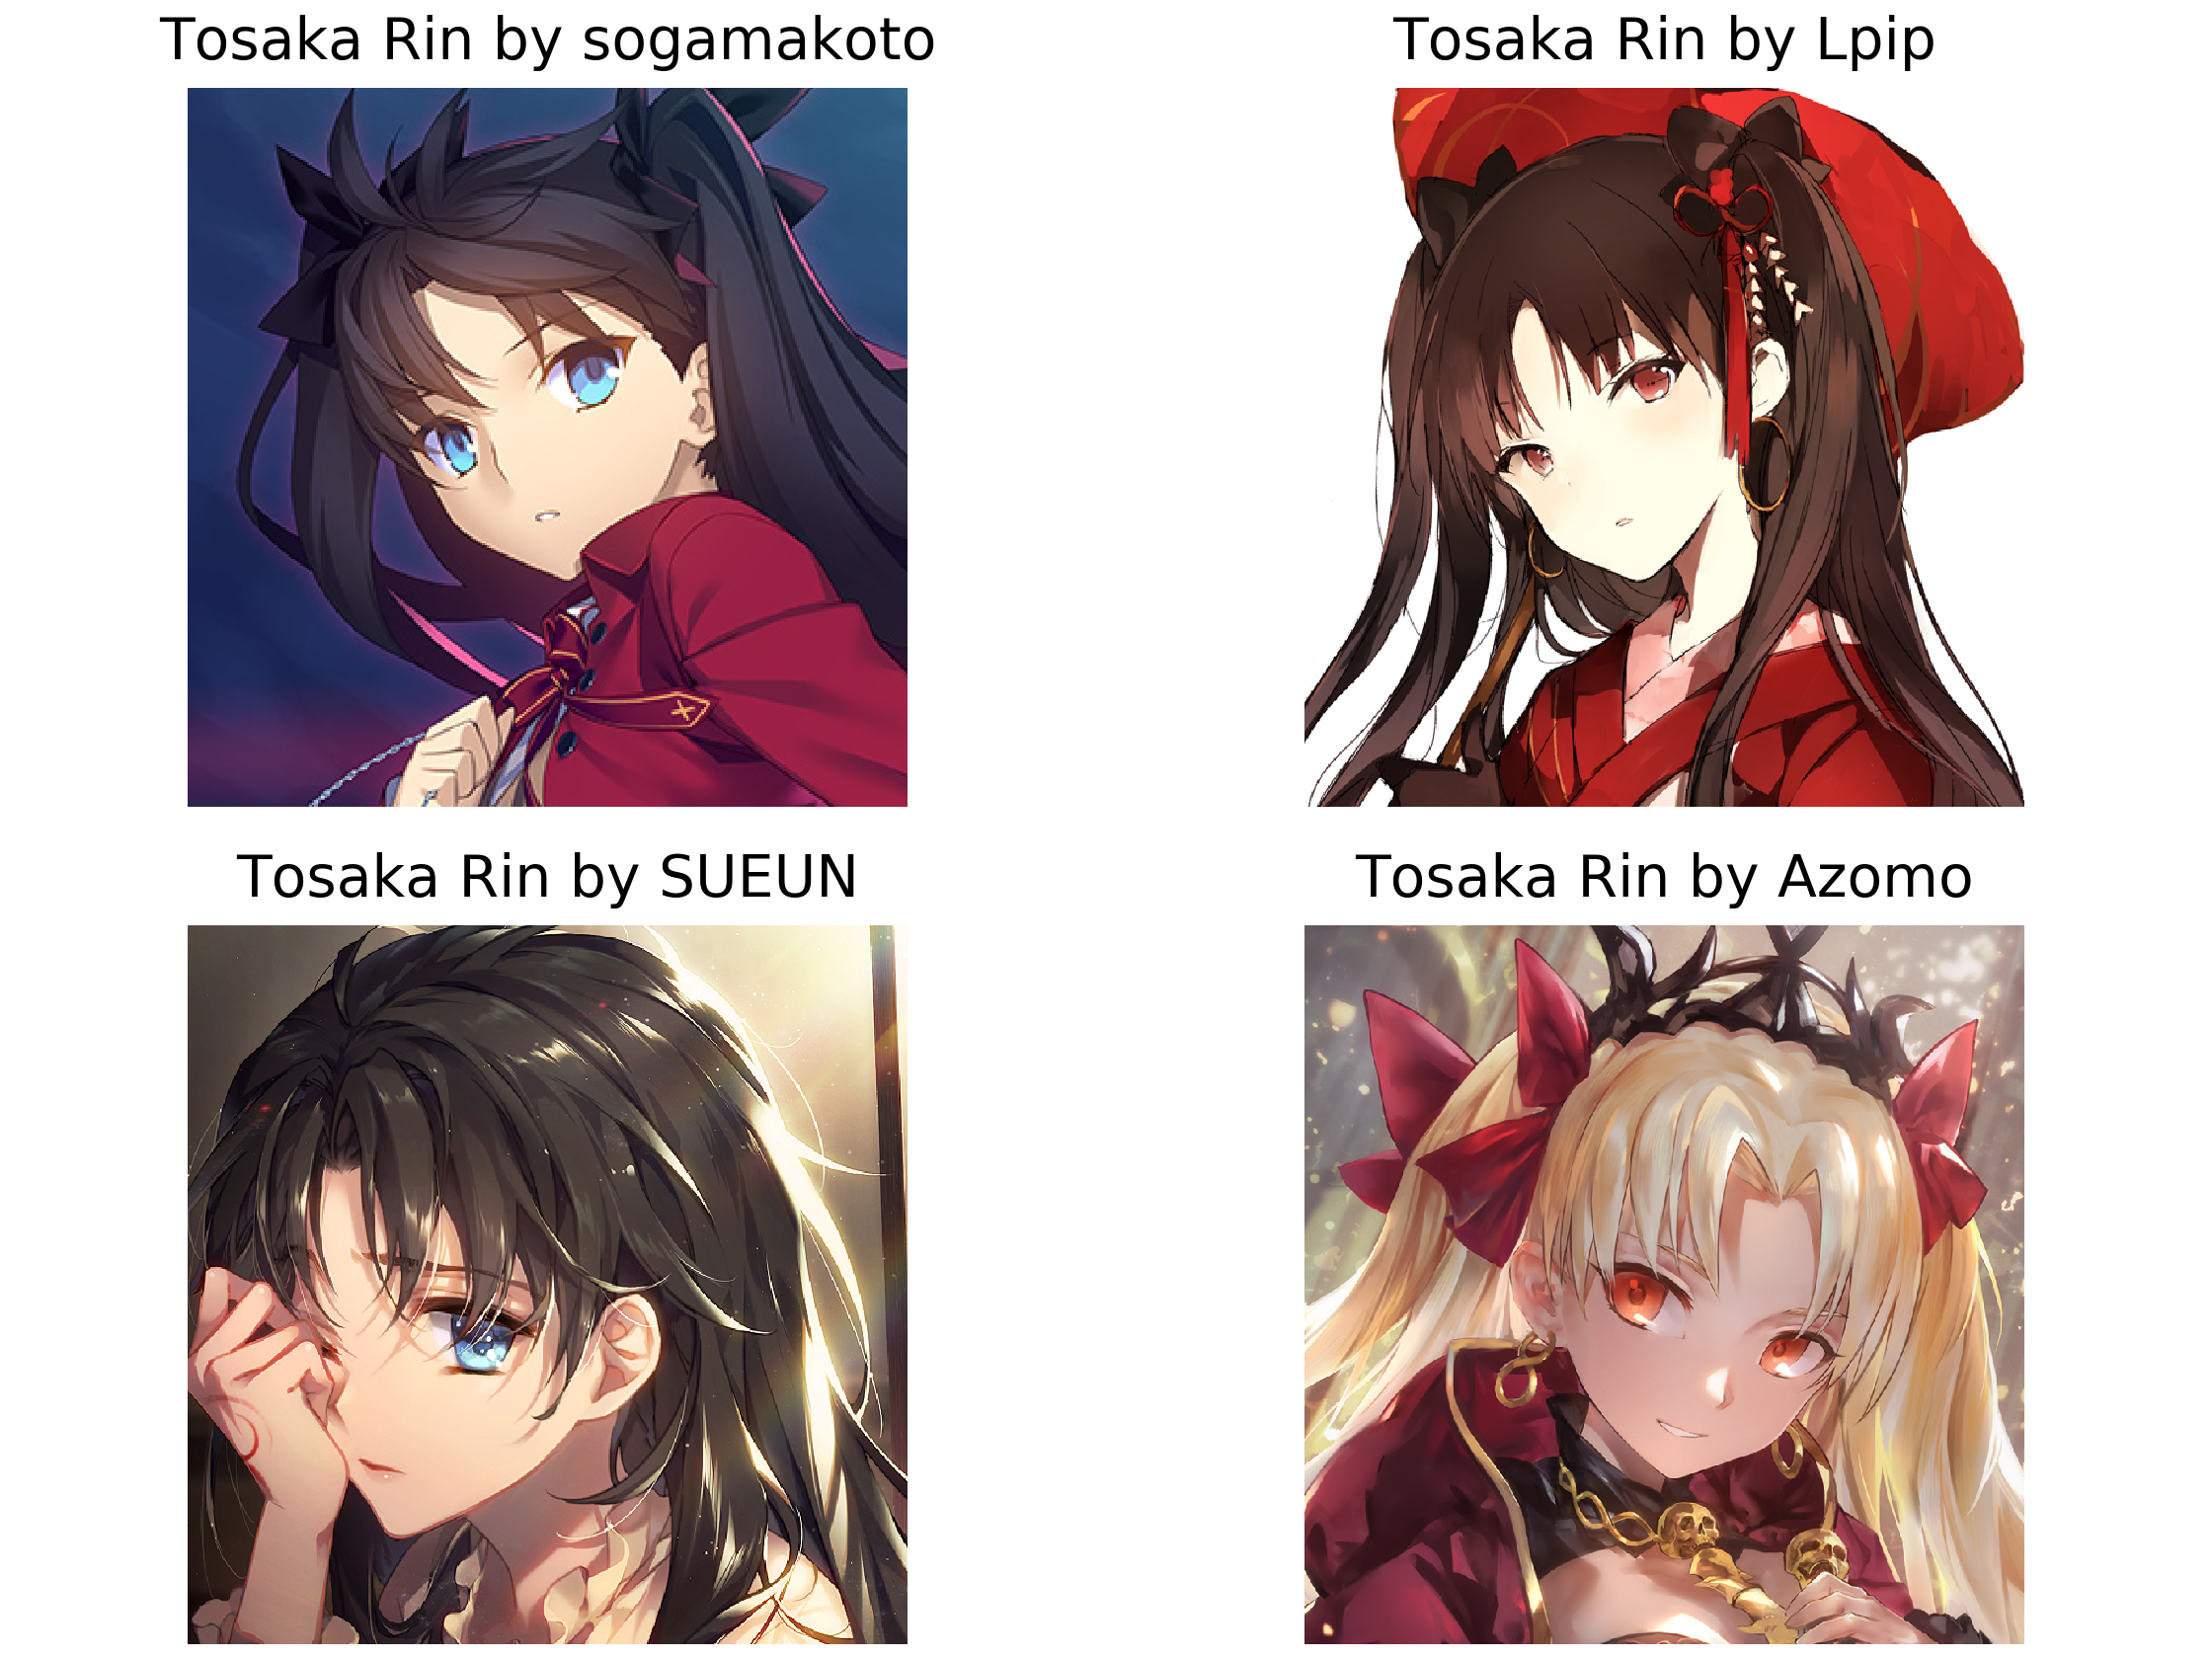
\includegraphics[width=0.8\linewidth, scale=1]{./images/tosaka_grid.png}
                    \caption{Same Character by different illustrators}
                \end{subfigure} & 
                \begin{subfigure}[h]{0.4\linewidth}
                    \centering
                    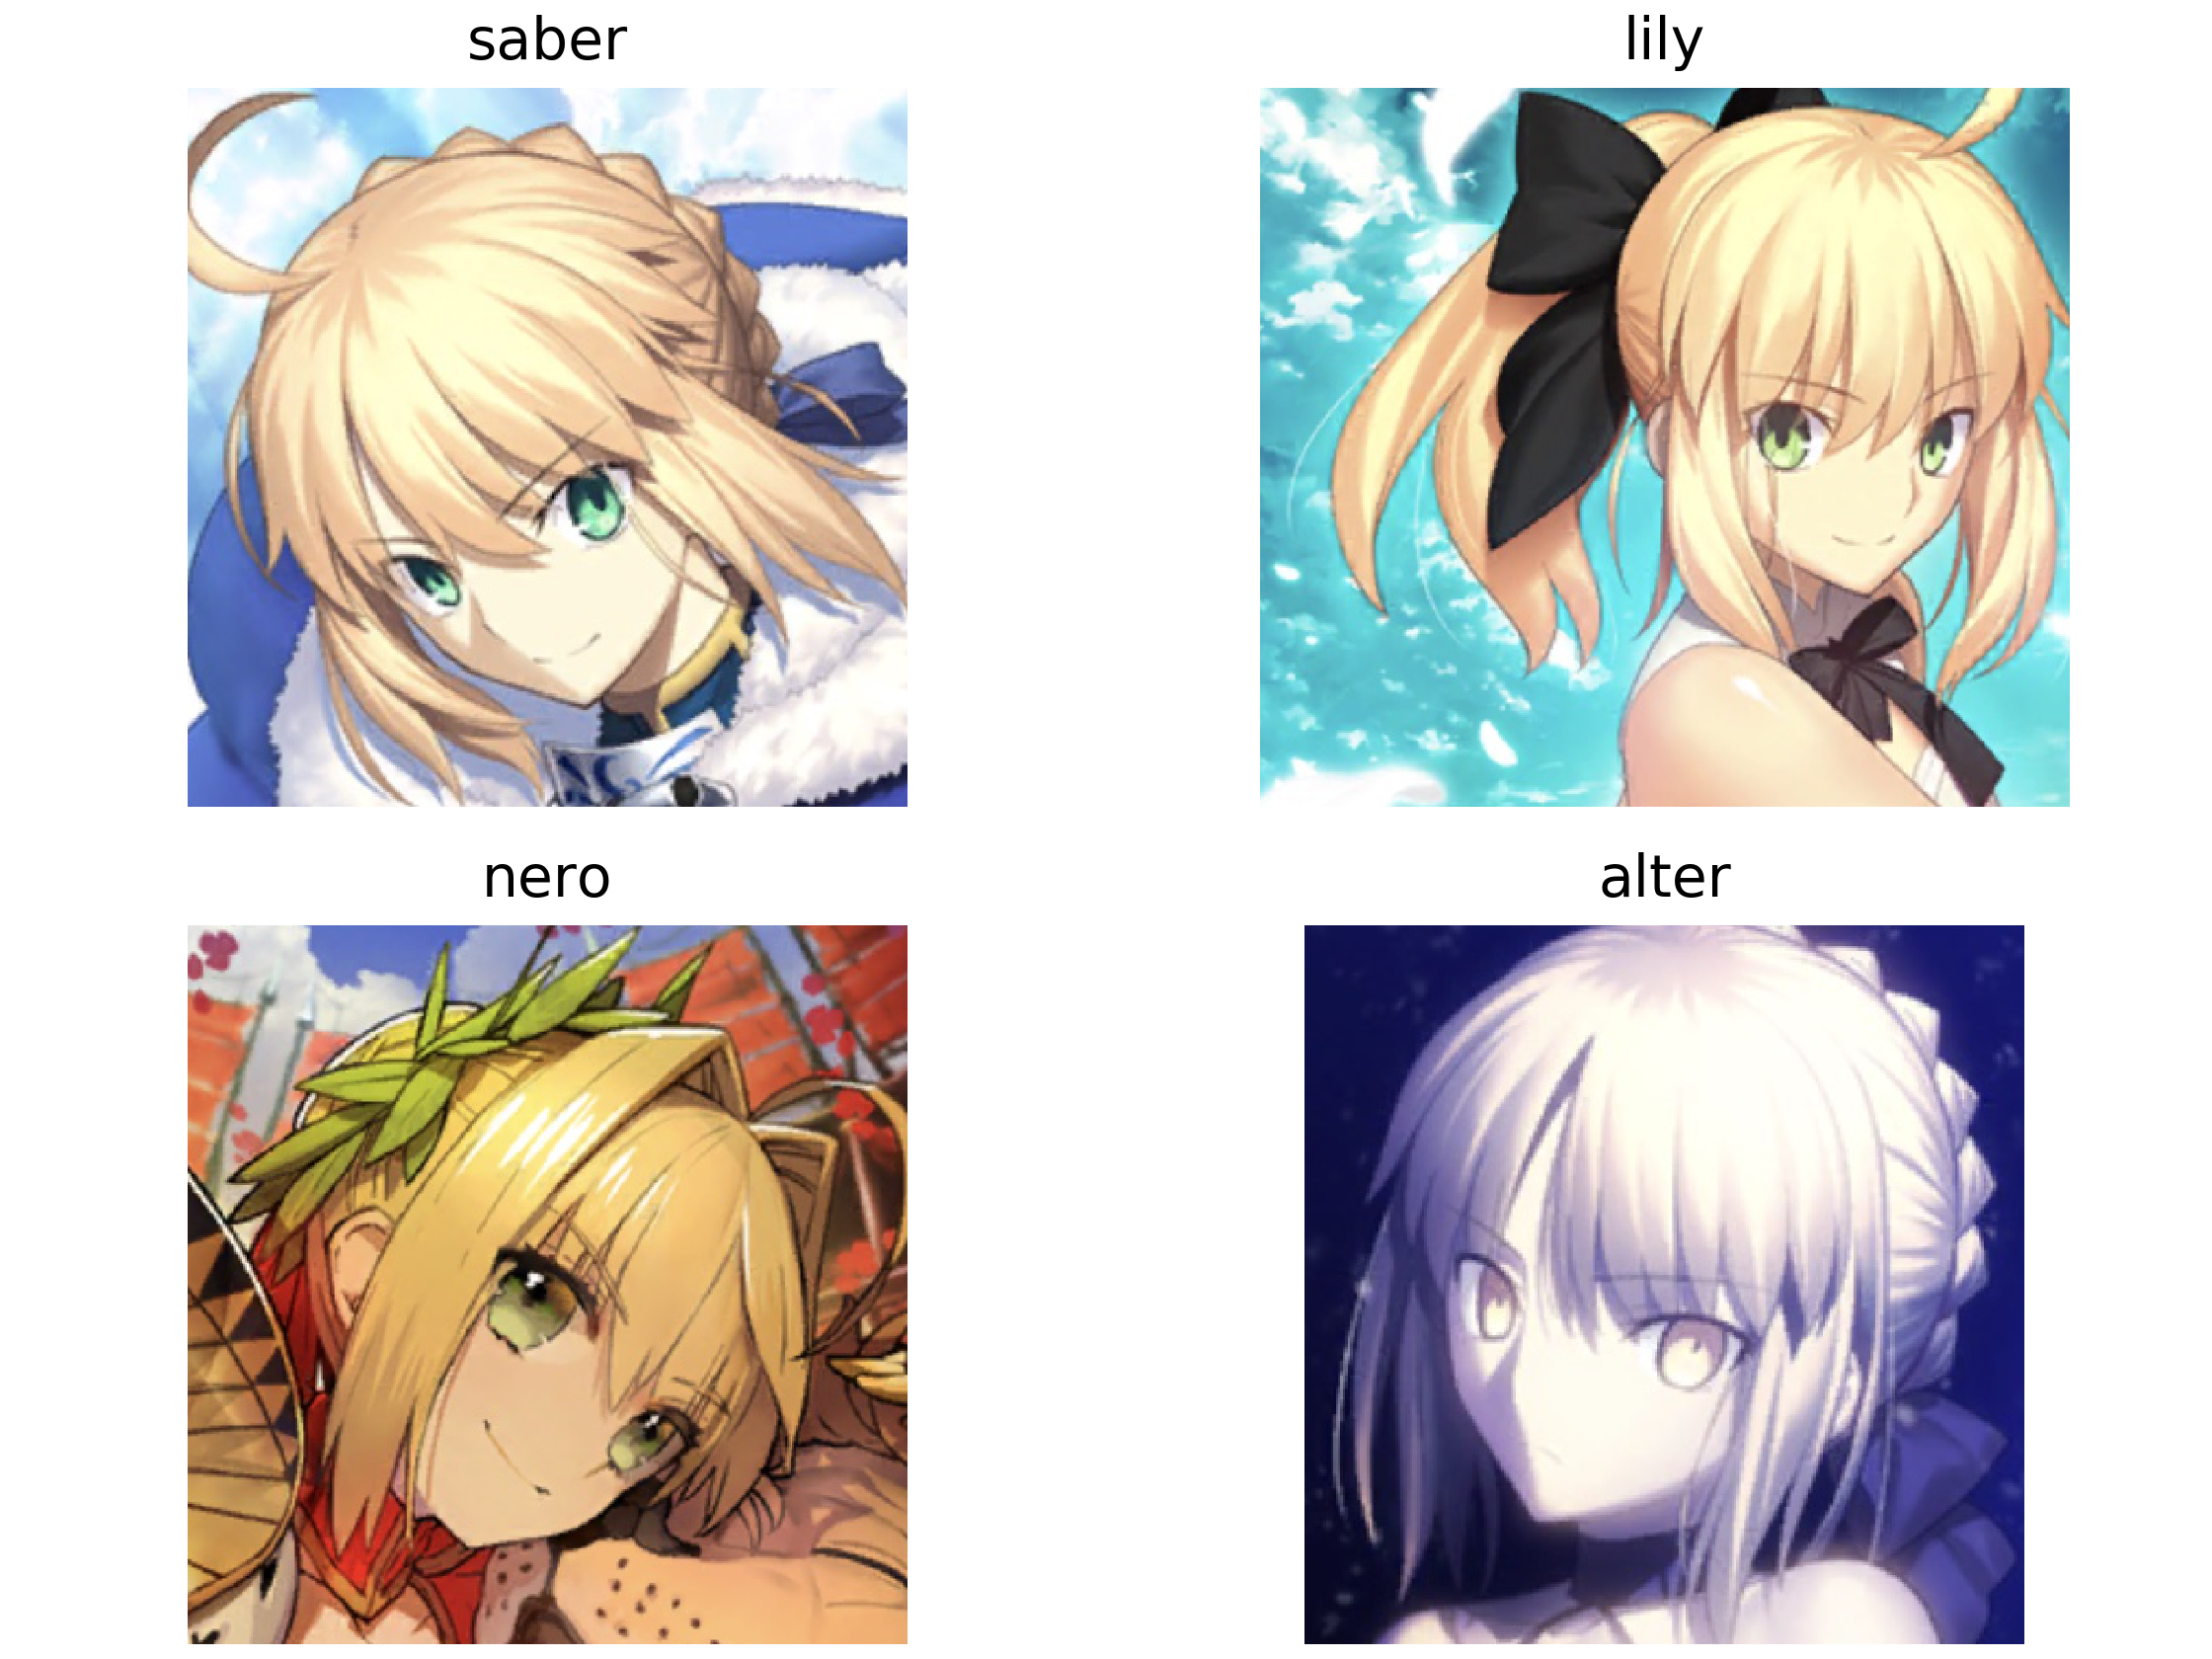
\includegraphics[width=0.8\linewidth, scale=1]{./images/saber_grid.png}
                    \caption{Similar characters}
                \end{subfigure}
            \end{tabular}
        \end{center}
        \caption{Various Looks of a Single Character and Similar but different Characters}
    \end{figure}
    \\ 
    Untagged illustrations would make some trouble for animation community members.
    Large number of 'Who is she/he' questions are emerging on social networks plantforms like Twitter, 2Chan and Bilibili.
    Even some video makers are posting works on answering those questions.
    On the other hand, within the machine learning community, if anyone is trying to make a illustration suggestion system based on the features or characteristics of anime characters, or trying to use GAN (Generative Adversarial Network) to generate fake anime illustrations, they might have to tag those pictures manually.\\ 
    Automatic character recognizing would then make some differences when one is facing a large set of untagged illustrations or would like to add/optimize tags based on character. For example, a character may be bounded to specific tags, like blond, green-eye, sword, armored, etc.
    This project is aiming to use machine learning techniques to automatically recognize characters in illustrations, based on their faces. We are mainly focusing on characters from japanese styled mangas and aminations. This project is making use of a variety of classification models including models like logistic regression classifier, random forest classifier and support vector machine and neural networks.\\ 
    In order to make it possible to train non-neural-network models, we performed feature extraction techniques on images during the preprocessing stage. The first strategy is extracting the texture, color and shape contents from the images and then flattern those features to an vector for the models to lean. The second strategy is extracting features using the output of the last layer of a pre-trained \texttt{ResNet}\cite{resnet} as the image features and train them on non-neural-network models.\\ 
    In this project, we did hyperparameter tuning on a rather small dataset that is collected manually by us and then train the model on the whole dataset which consists of ours and Nagadomi's anime face character dataset\cite{dataset}. Neural network performed best with a recognition rate of 90\%. Support vector machine was the best model among non-neural-network models with \texttt{ResNet}\cite{resnet} extracted features. 


    \section{Technical Approach}
    % Please describe the techniques you have used in order to address the problem.
    % Describe in detail the classification/regression/other techniques you have used in order to tackle the problem.

    In this project, we made use of techniques relating to image feature extractions, classification models and neural networks to tackle the animation image classification problem.

    \begin{enumerate}
        \item \textbf{Feature Extraction Algorithms}
        
        Initially, we naively flatterned the RGB channels of a image to a vector as the input of the models, but find out that about 5-15 minutes are required to train a model even on the small dataset collected by ourselves. Additionaly, the prediction is not accurate since the flatterning process destroies the spacial relation between each pixels. Therefore, we find some way to extract the features of a image.
        \begin{itemize}
            \item \textbf{Image Moment}
            
            Image moment is a certain particular weighted average of the image pixels' intensities. A uniqueness theorem \cite{img_moment} claim that a piecewise continuous 2D function $f(x,y)$ with nonzero values in a finite part of the $xy$ plane, then moments of all orders exist and moment sequence is uniquely determined by $f(x,y)$. Image moments are useful to describe the shape of a image content. In this project, we made use of pre-implemented function $hu\_moment()$ in \texttt{OpenCV}\cite{opencv_library} to process the image.
            \item \textbf{Haralic Texture}
            
            Haralic texture, proposed by R. M. Haralick et al. in 1973, is describing a textural features "based on graytone spatial dependancies" \cite{haralick}. This algorithm is trying to conclude the texture of a surface and the "structural arrangement of surfaces and their relationship to the surrounding environment"[]. In this project, we made use of the algorithm to extract the texture information of the images. The extraction of Haralic Textures is implemented in python package \texttt{mahotas}\cite{mahotas}, with function $mahotas.features.haralick()$
            \item \textbf{Histogram of Colors}
            
            In order to zip the information of color of a image, we decide to calculate how color are ditributed in $HSV$ channels. To discretize the continuous distribution of colors, we decide to use 8 bins in each channel and thus store the histogram of colors to a vector. Again, we made use of \texttt{OpenCV}\cite{opencv_library} to process the image.
        \end{itemize}
        \item \textbf{Prediction Models}
        
        In this project, we made use of many of the models that we learned in this course as well as some models in the prerequisite of this course. The implementation of these models are from python package \texttt{scikit-learn}\cite{scikit-learn}. 
            \begin{itemize}
                \item \textbf{Logistic Regression}
                
                Logistic regression is used to model the probability of a certain class. With the feature input $x \in \mathbf{R}^n$, calculate $w^Tx + b, w \in \mathbf{R}^n, b \in \mathbf{R}$ the probability of $x$ in certain class is denoted by 
                $p(x = X | w) = \frac{1}{1 + e^{-(w^Tx + b)}}$
                In order to tacle overfitting problem, we also add a regularization strength $\lambda$. $\lambda$ is a hyperparameter need to be determined before training. Training logistic regression is through gradient descent. In \texttt{scikit-learn}\cite{scikit-learn}, this problem is formed as a optimization problem: 
                $\min_{w, c} f(w) + c\sum_{i=1}^{n}\frac{1}{1 + e^{-y_i(w^Tx_i + b)}} $ 
                where $f(w) = ||w||^2_2$ if we choose $l_2$ penalty.\\ 
                In order to enable the model to classify multi-labels data, we train $k$ models for $k$ labels. Each model is a "one-vs-rest" classifier. When testing a given input, just find out the highest probability of all models and assign its class to the input.
                \item \textbf{Linear Discriminant Analysis}
                
                Linear discriminat analysis(LDA) is a Fisher's linear discriminant\cite{fisherDA}. It is closely related to analysis of variance (ANOVA) and regression analysis. LDA assumes that the conditional probability density functions are normally distributed and the class covariances are identical.           In this project, we uses multiclass LDA. This multiclass generalization is due to C. R. Rao\cite{multiLDA}. Also, we directly use the implemented model from \texttt{Scikit-learn}\cite{scikit-learn}

                \item \textbf{k-nearest neighbors}
                
                $k$-nearest neighbors(kNN) is a non-parametric passive model used for classification. Upon an input object, the model classify by a vote of its neighbors. The most often appeared class in its $k$ nearest neighbors are the output class. $k$ is a hyperparameter that we need to decide before the training.
                \item \textbf{Decision Trees}
                
                Decision Trees are a non-parametric supervised learning method used for classification. The model is in a tree structures where its leaves represent class labels and branches represent conjunctions of features that lead to those classes. In this project we directly use the Classification and Regression Tree (CART) implemented in \texttt{scikit-learn}\cite{scikit-learn}.
                \item \textbf{Random Forest}
                
                Random Forest is constructing a mutiple decisions trees at training time and outputting the class that is the mode of the classes of individual trees. This method is first proposed by Tin Kam Ho in 1995\cite{random_forest}. Training process, called bagging\cite{rf_bagging}, is repeatly select a random sample with replacement of the training set and fits a decision tree with these samples. We made use of the $RandomForestClassifier$ of \texttt{scikit-learn}\cite{scikit-learn} to perform the classification job.
                \item \textbf{Gaussian Naive Bayes}
                
                Naive Bayes is based on applying Bayes theorem with assumptions of features are mutually independent with each other. In multi-class classification, we can calculate the value of the probability of all classes of a given input under the naive bayes assumption and find the class with the highest probability. Gaussian Naive Bayes is just making the assumption that the features are normally distributed. 
                \item \textbf{Support Vector Machines}
                
                Support Vector Machines(SVMs) are supervised learning models used for regression and classification problems. With the assumption that the data is seperatable with a hyperplane, SVM is trying to find the hyperplane with the maximized margin between the data point in each class and the hyperplane.
                We made use of the C-Support Vector Classification (SVC) provided by \texttt{scikit-learn}\cite{scikit-learn}. We selected the "one-vs-one" scheme during the training. Hyperparameters need selection: regularization parameter $C$, kernel funciton, and the degree of polynomial kernel(if polynomial function is selected as kernel).
            \end{itemize}
        \item \textbf{Neural Networks}
        
        Neural Networks(NN), first introduced by Warren McCulloch and Walter Pitts\cite{nn_init} are computing structures inspired by biological neural networks. This system is composed of several layers of artifical neurons that mimics the firing of biological neurons. \\
        In this project, we used \texttt{pytorch}\cite{pytorch} to form and train neural networks. Particularly, we borrowed the \texttt{ResNet}\cite{resnet} that is pre-trained on \texttt{ImageNet}\cite{imgnet} and added a layer of neurons representing our class labels and trained the net with our dataset.
    \end{enumerate}


    \section{Experimental Results}
%    Describe the datasets used for your experiments. Be precise in describing all information about the datasets, including, classes, number of samples per class, features used to represent data, and all pre/post processing of the datasets.\\
%    Describe the details about the implementation of each algorithm, e.g., how you perform training, validation, testing, values of the hyperparameters and your methods for hyperparameter tuning, training/validation/testing error on the dataset, and all useful plots/tables that help to better interpret your results and your work.\\ \\
    \begin{minipage}{0.5\textwidth}
        In this project, we have gone through a working pipeline shown in Figure 3.
        Firstly, we manually cleaned the Nagadomi's Anime Face Character Dataset and generated our own dataset with better image quality and modern animation characters.
        Then, we performed image pre-processing and feature extractions to generate three union of data: color-texture-shape information, ResNet-processed information and normalized RGB information.
        Then we designed different models according to these unions of data.
        
        According to our models, we did hyperparameter tuning on the self-collected dataset and then trained the model with the optimized hyperparameter on the whole dataset and evaluate the prediction result.
        Following are the detailed description of each step in the working pipeline.
    \end{minipage}
    \begin{minipage}{0.5\textwidth}
        \begin{center}
            \textbf{Working Pipeline}
        \end{center}
        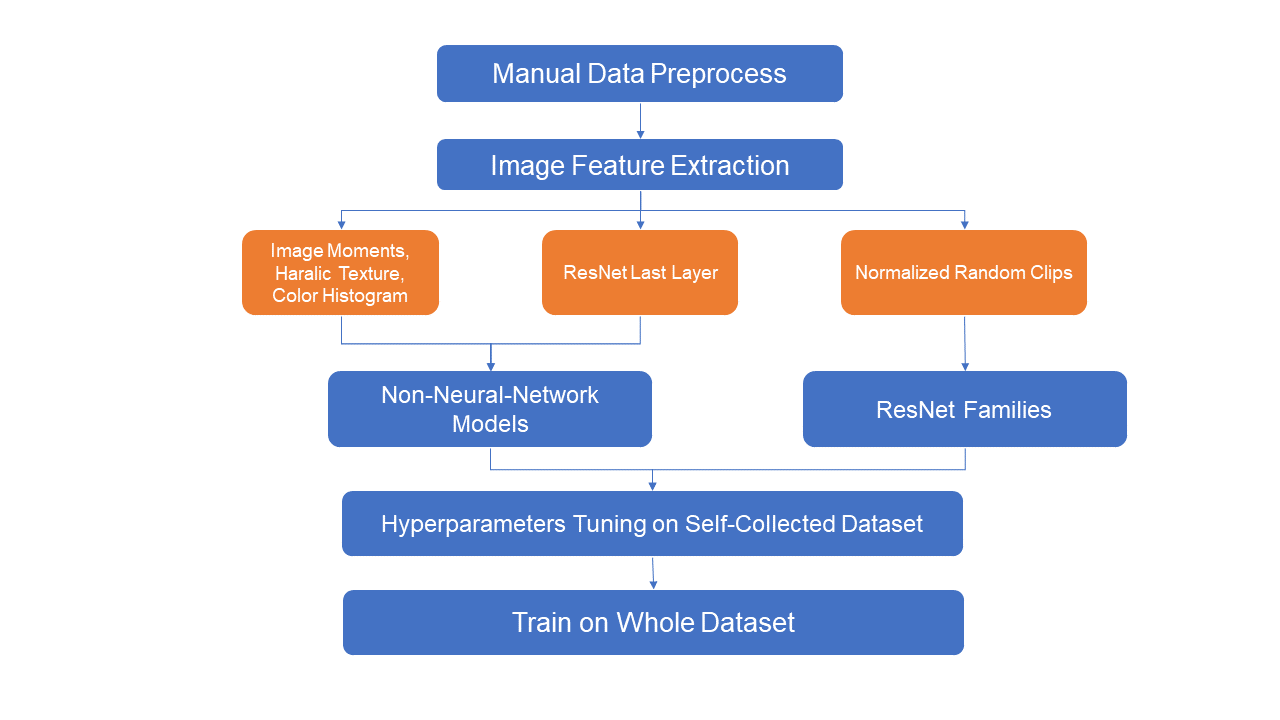
\includegraphics[width=\textwidth]{images/working_pipeline.png}
    \end{minipage}

    \begin{enumerate}
        \item \textbf{Dataset Overview}
        \begin{itemize}
            \item \textbf{Nagadomi's Anime Face Character Dataset}

            Nagadomi's dataset contains 173 different animation characters.
            Most of the classes contains more than 50 images.
            However, it was collected 6 years ago, there are some problems in the dataset.
            Many of the characters are out of date so that fan art on them are no longer active.
            Also, most of the image size is around 100 * 100 pixels which are considered low resolution in modern standard.
            Therefore, some of them are difficult even for a senior community member to recognize.
            Furthermore, there exists some falsely labeled images, For example, shown in Figure 2, many pictures of Meirin Ri was labeled as Daidouji Tomoyo.
            Lastly, the data is in baised in some extend i.e. some of the classes do not contain sufficient amount of data, especially those non-popular characters.
            Therefore, we did a manually filtering process to delete bad images like ones shown in Figure 2.
            A copy of filtered data is stored separately.
            \begin{figure}[h!]
                \centering
                \begin{tabular}[c]{cccc}
                    \begin{subfigure}[h]{0.2\linewidth}
                        \centering
                        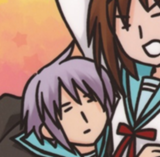
\includegraphics[width=0.5\linewidth, scale=0.5]{images/face_145_303_113.png}
                        \caption{Bad Nagato Yuki}
                    \end{subfigure} &
                    \begin{subfigure}[h]{0.2\linewidth}
                        \centering
                        
\includegraphics[width=0.5\linewidth, scale=0.5]{images/face_235_235_128.png}
                        \caption{Good Nagato Yuki}
                    \end{subfigure} &
                    \begin{subfigure}[h]{0.2\linewidth}
                        \centering
                        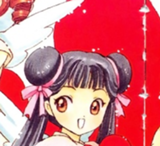
\includegraphics[width=0.5\linewidth]{images/face_795_301_69.png}
                        \caption{Meirin Ri labeled as Daidouji Tomoyo}
                    \end{subfigure} &
                    \begin{subfigure}[h]{0.2\linewidth}
                        \centering
                        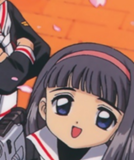
\includegraphics[width=0.5\linewidth]{images/face_1141_433_41.png}
                        \caption{Real Daidouji Tomoyo}
                    \end{subfigure}
                \end{tabular}
                \caption{Problematic Data Entry Examples}
            \end{figure}
            \item \textbf{Self-collected Dataset}

            Due to the drawbacks of the existing dataset, we also collected some images with better quality.
            Totally, we collected images of 7 characters, each with over 100 images, manually from animations and illustrations published on web.
            These images are in similar format as images in Nagadomi's dataset, square-like images of faces of anime characters but with higher resolution (about 400 * 400) and better quality (high quality fan-arts).
            \item \textbf{Subset-ing the whole dataset}

            After the manual filtering process, there remains 163 characters.
            Since it was impracticable to train our models and tune hyperparameters using all of the data due to lack of computing power and time, we decide to manually pick a subset of characters from the whole dataset, each with over 100 images, to tune hyper-parameters.
            The training and testing on the whole dataset was performed on the tuned hyperparameter and the results will be reported.
            See Appendixes for the number of images in each class.
        \end{itemize}
        \item \textbf{Non-Neural-Network Models with Image Features inputs}
        \begin{itemize}
            \item \textbf{Data Pre-processing and Feature Extraction}

            This feature extraction process was a direct combination of HuMoments (implemented in texttt{OpenCV}\cite{opencv_library}), Haralick features (implemented in \texttt{mahotas}\cite{mahotas}), and color histogram (implemented in texttt{OpenCV}\cite{opencv_library}).
            The result of the previous feature extraction was plugged as input into the next feature extraction method.
            The order of feature extraction we chose was: HuMoments $\rightarrow$ Haralick $\rightarrow$ color histogram.
            \item \textbf{Model implementation}

            We have trained logistic regression(LR) classifier, linear discriminant analysis(LDA) classifier, K neareast neighbors(KNN) classifier, decision tree(CART) classifier, random forest(RF) classifier, Gaussian Naive Bayes(NB) classifier, and support vector machine(SVM) classifier all using \texttt{scikit-learn}\cite{scikit-learn} to tune hyper-parameters on the subset described above.
            \item \textbf{Hyperparameter Tuning}
            Hyperparameters was tuned using the subset of dataset described above and the result using all of our data would also be produced after hyperparameters was tuned.
            \begin{enumerate}
                \item Logistic Regression classifier

                Since we chose to use "lbfgs" solver in scikit-learn, we can only use l2-norm in penalization, or use no regularization.
                Logistic regression models with or without regularization functions and with different regularization strength used in penalty function (C in scikit-learn) was trained to find out whether we are regularizing and the value of regularization strength.
                The regularization strength, C, was tested with floats ranging from $0.1$ to $10.0$ to find the best value.

                Testing results:

                \begin{figure}[h!]
                    \centering
                    \begin{tabular}[c]{cc}
                        \begin{subfigure}[h]{0.4\linewidth}
                            \centering
                            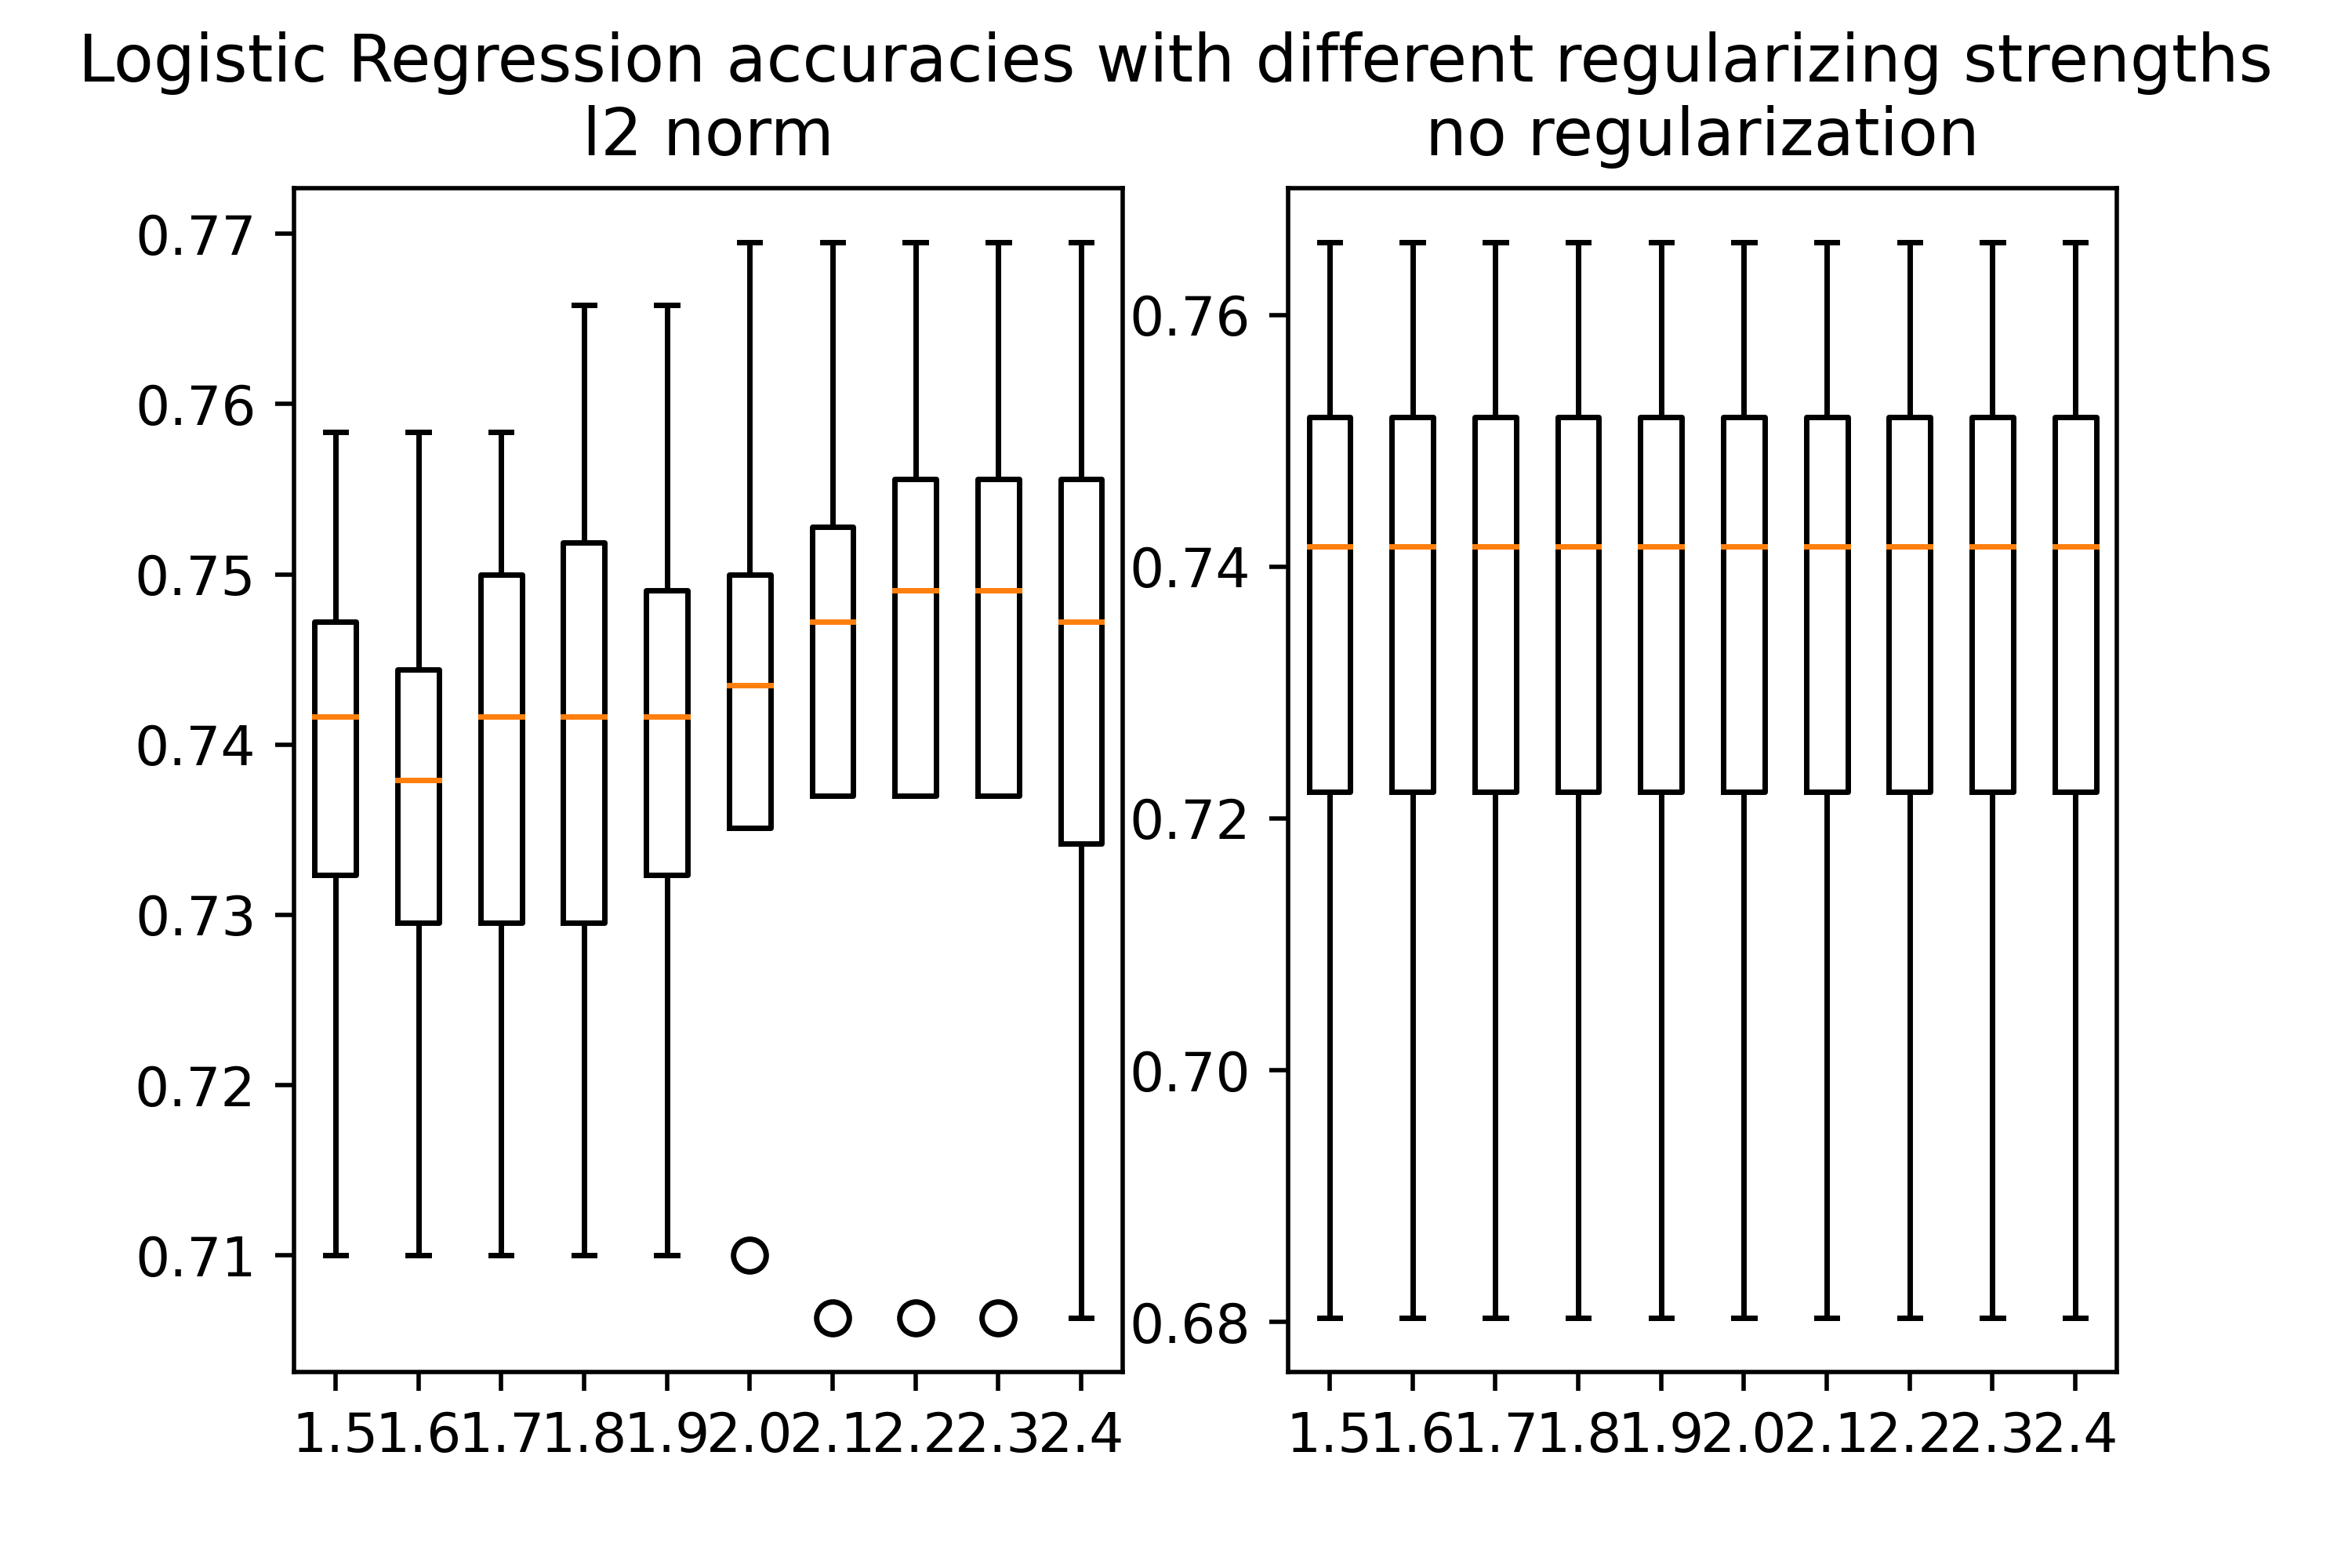
\includegraphics[width=0.75\linewidth]{images/log_reg_hyperparam_penalty.png}
                        \end{subfigure} &
                        \begin{subfigure}[h]{0.4\linewidth}
                            \centering
                            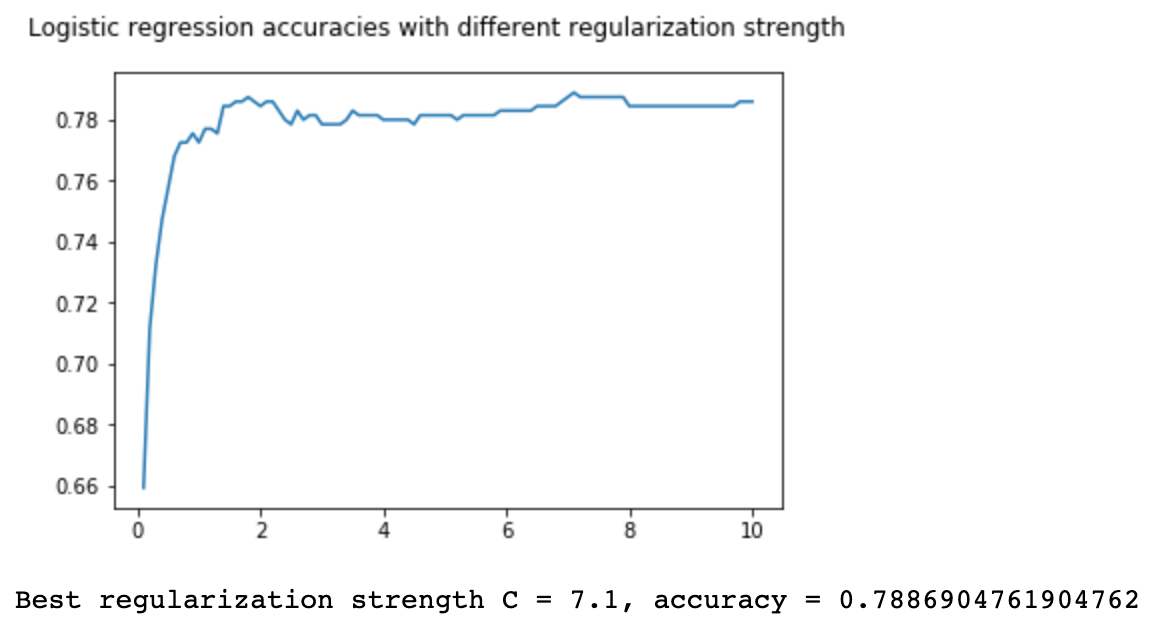
\includegraphics[width=0.75\linewidth]{images/log_reg_hyperparam_c.png}
                        \end{subfigure}
                    \end{tabular}
                    \caption{LR on Image Features hyperparameter tuning}
                \end{figure}
                As shown in the result, we should have l2-norm regularization in penalty function, and the best regularization strength $C= 4.5$, with accuracy $= 0.807$

                \item K Nearest Neighbors classifier

                We tried out different values of $k$, ranging from $2$ to $30$ to find the best value of $k$.The $k$ performing the best is $k = 6$.
                % Testing results:
                % \begin{figure}[h!]
                %     \begin{subfigure}[b]{\linewidth}
                %         \centering
                %         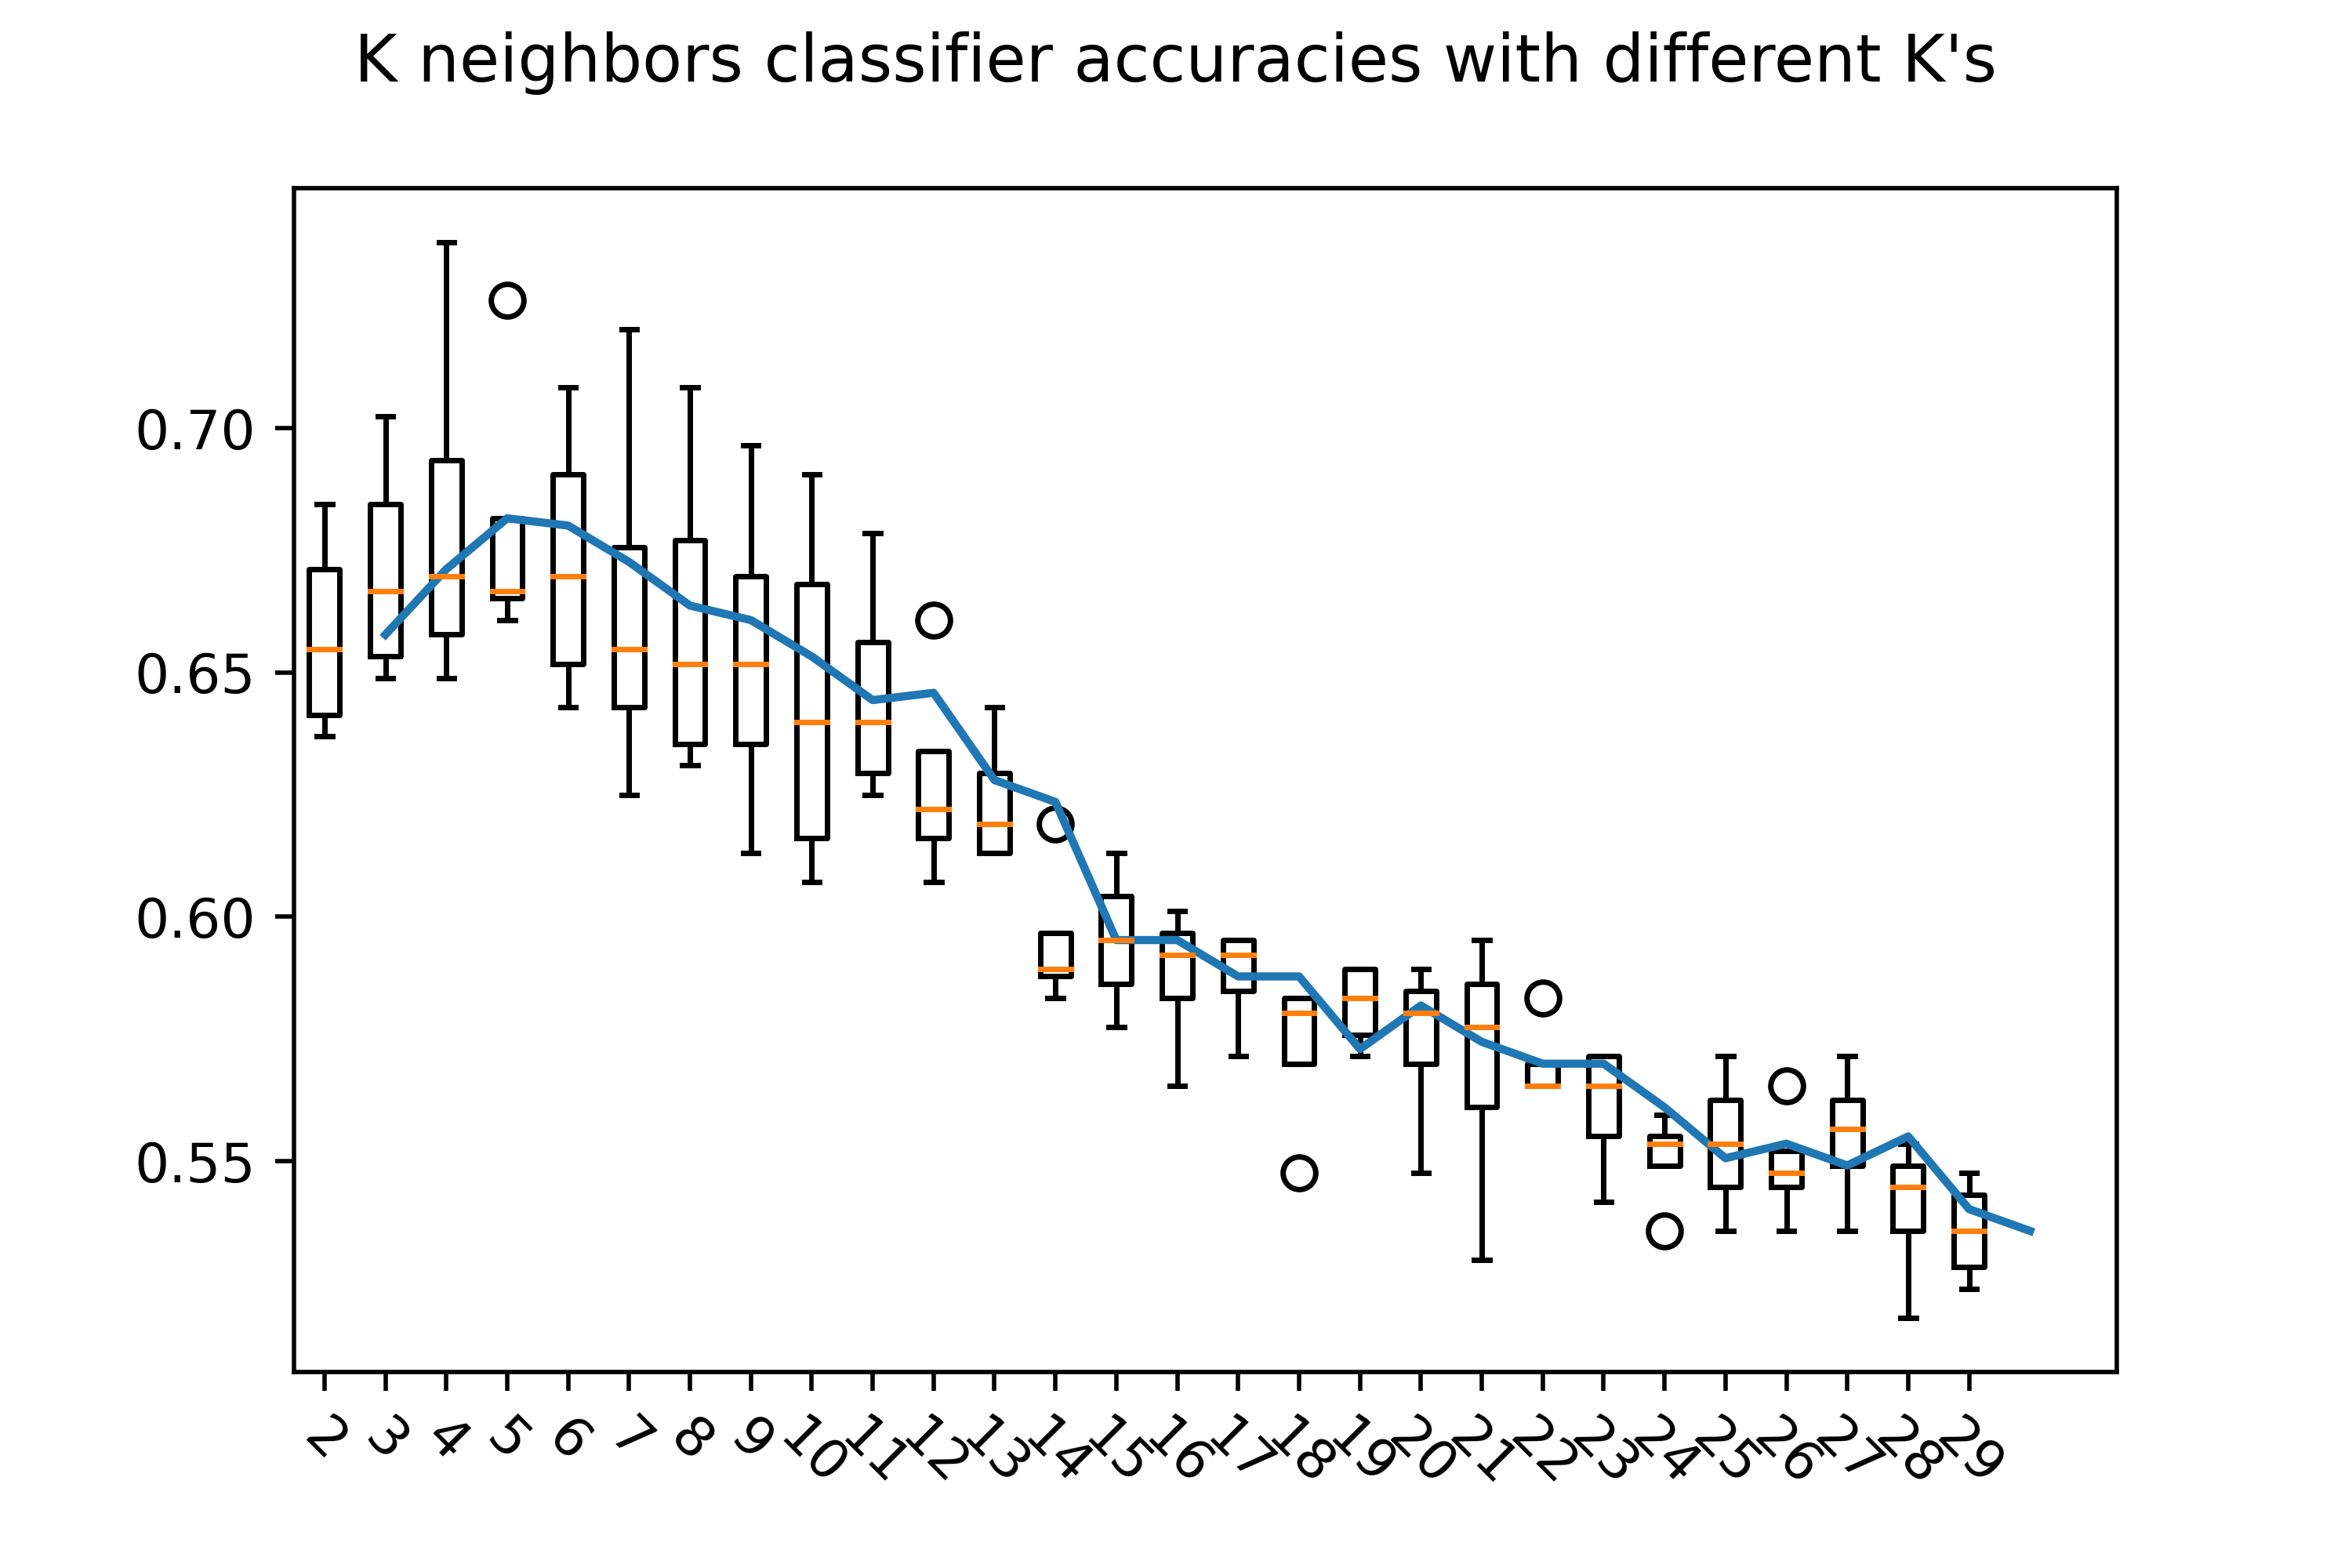
\includegraphics[width=0.5\linewidth]{images/knn_k.png}
                %     \end{subfigure}
                %     \caption{K Neighbor classifiers hyperparameter tuning}
                % \end{figure}
                \item Random Forest classifier

                We have tried forests with different loss function, Gini impurity function and Information Entropy function, both accuracy and computing time was record:

                \begin{figure}[h!]
                    \begin{subfigure}[b]{0.5\linewidth}
                        \centering
                        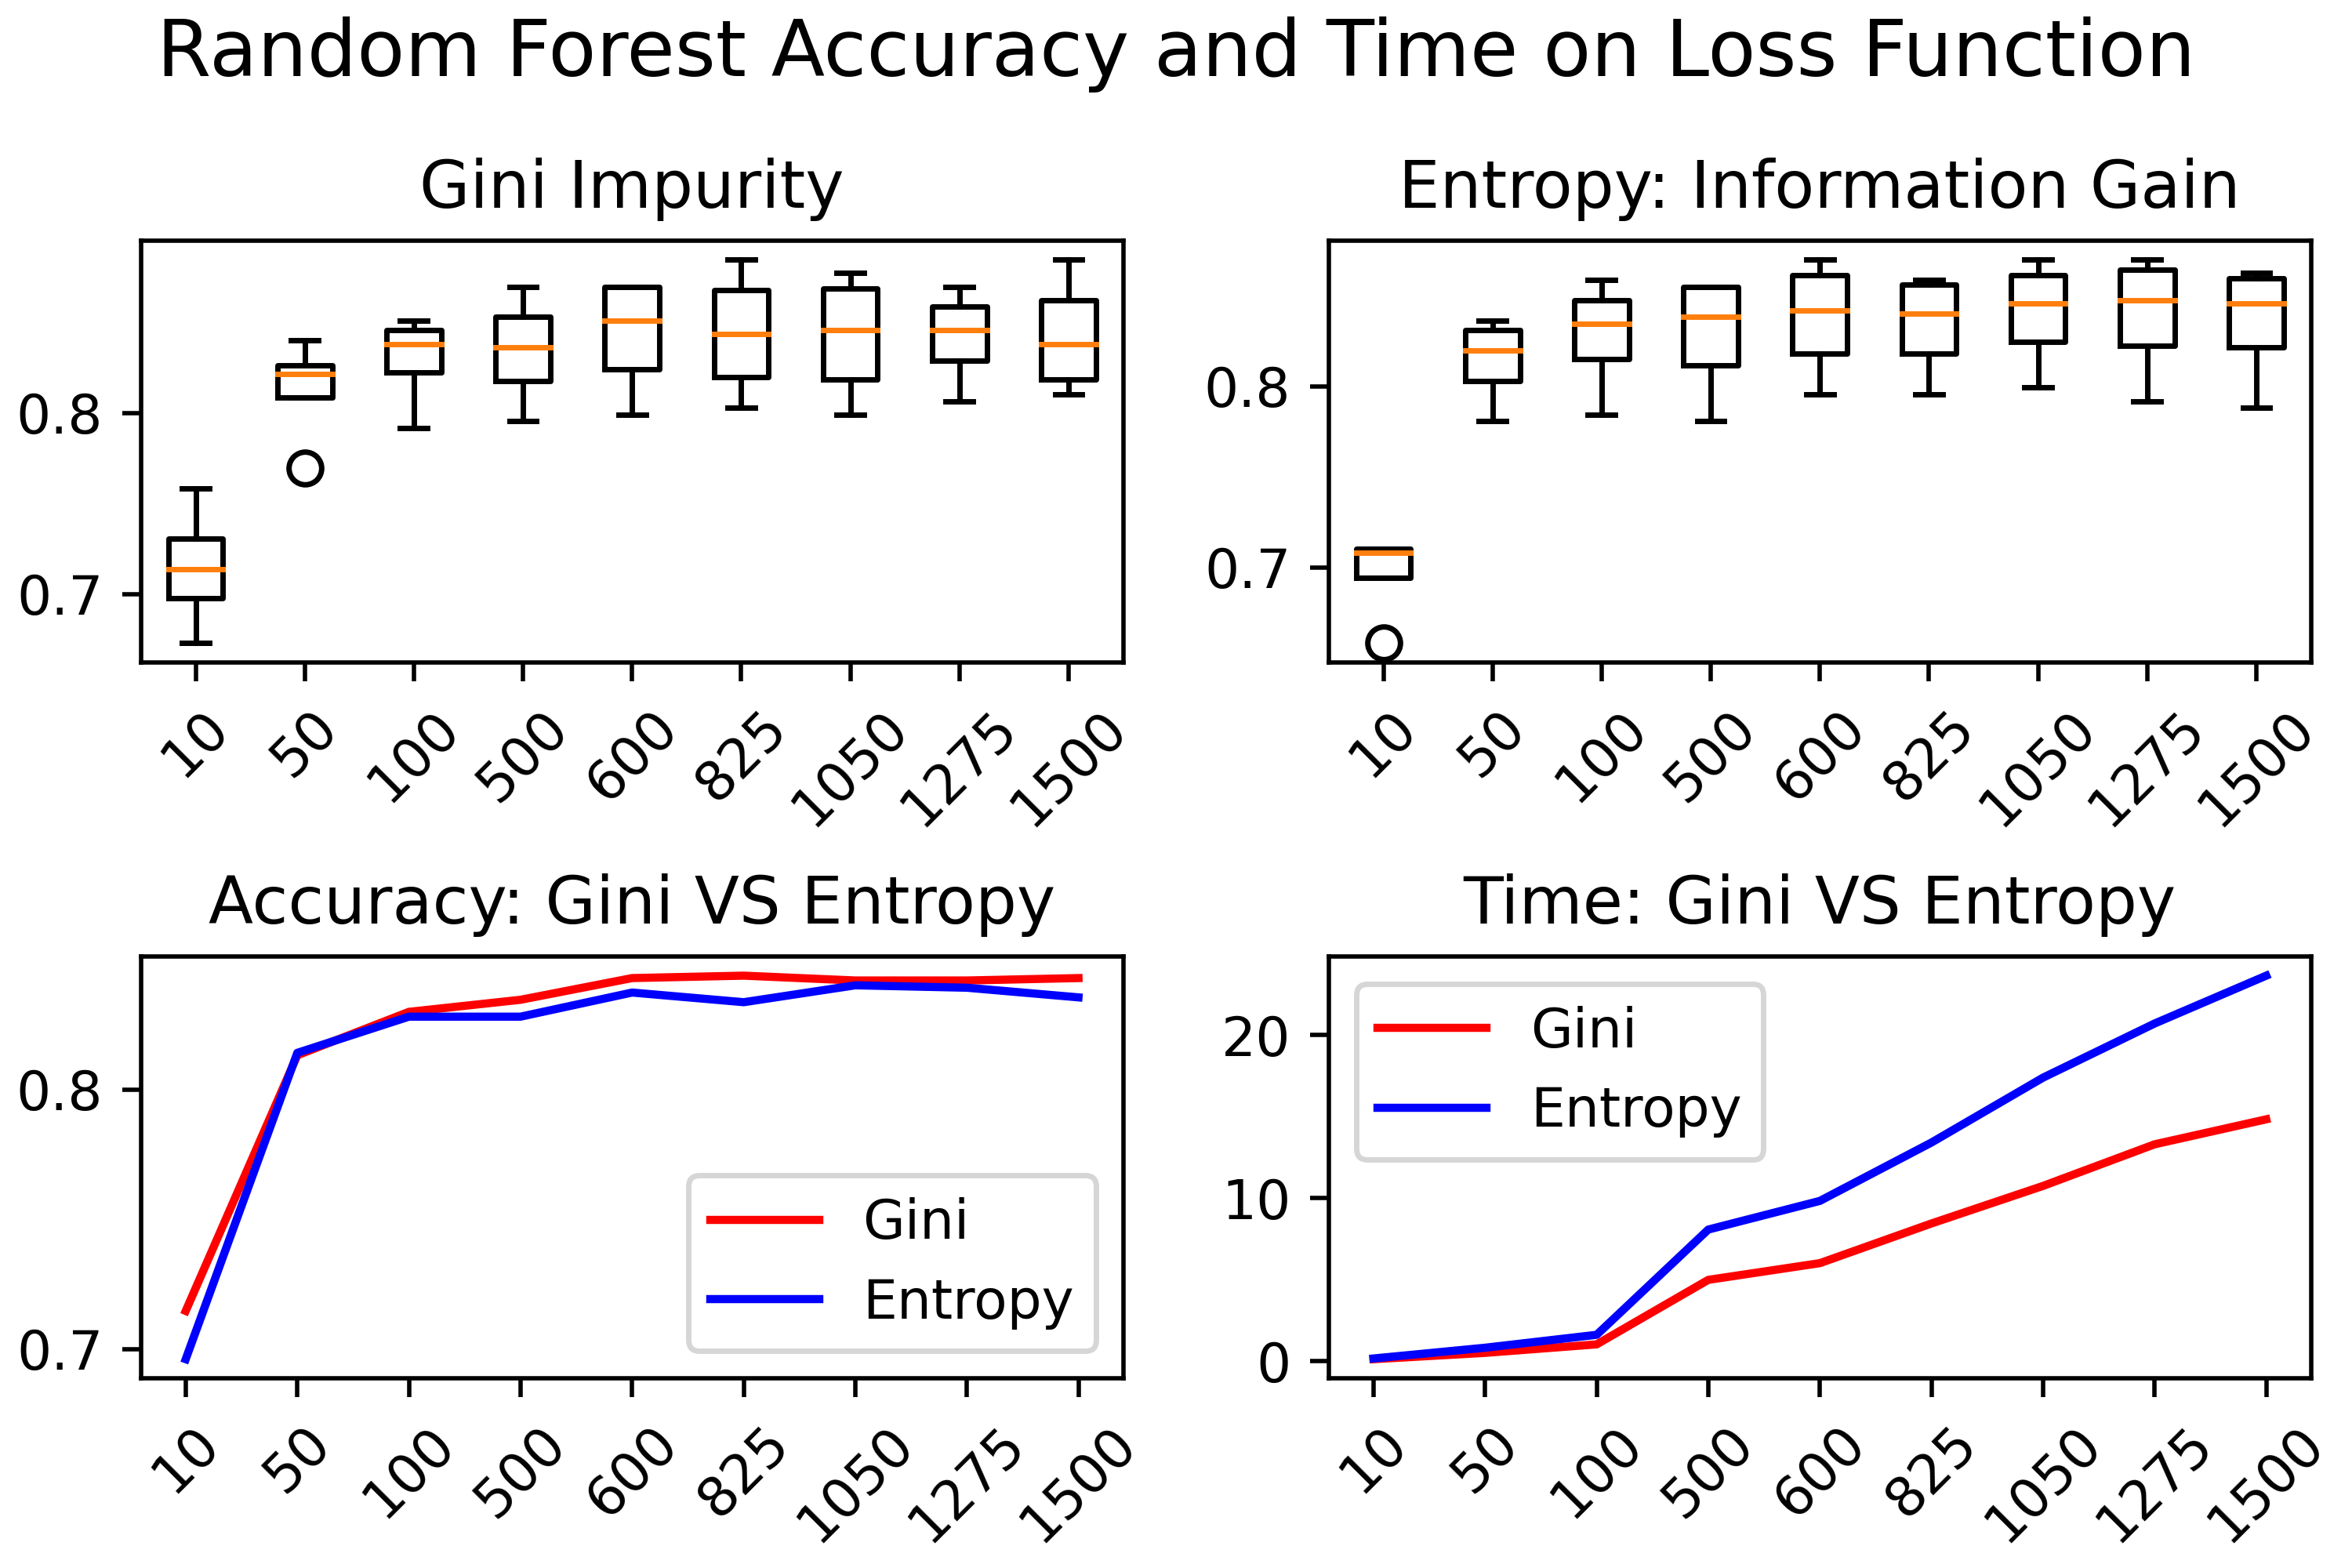
\includegraphics[width=0.75\linewidth]{images/rand_forest_loss_func.png}
                    \end{subfigure}
                    \begin{subfigure}[b]{0.5\linewidth}
                        \centering
                        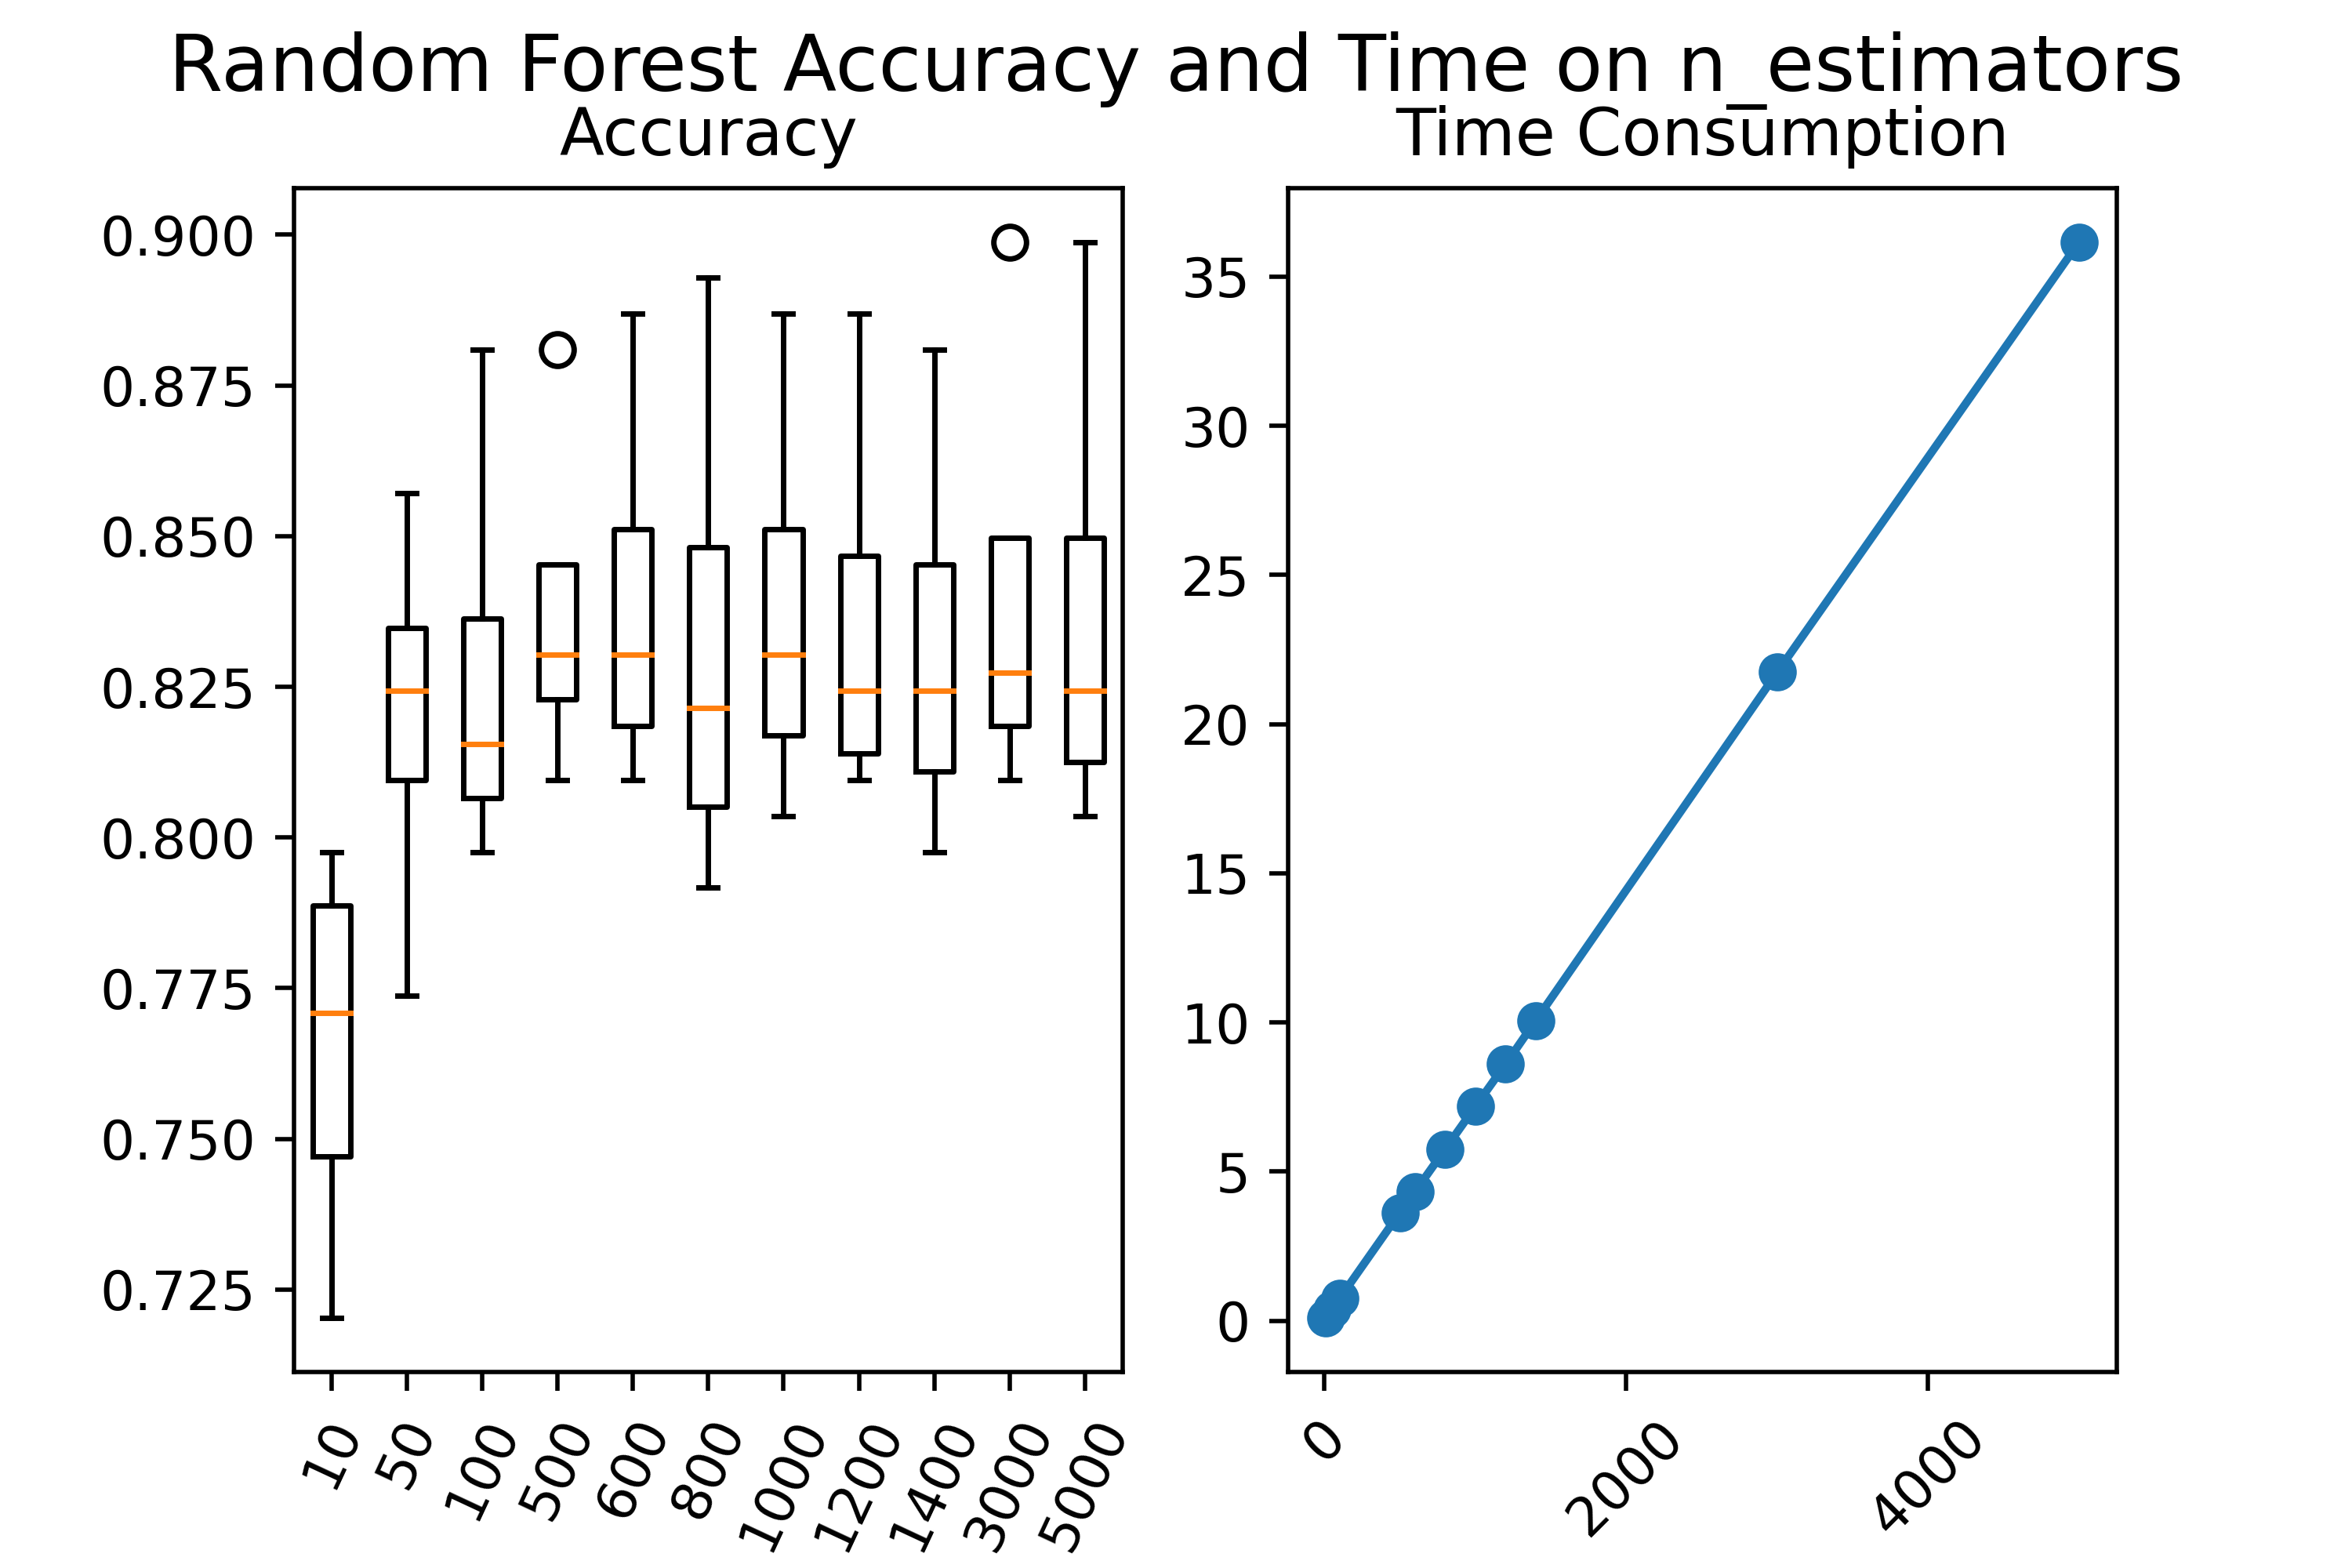
\includegraphics[width=0.75\linewidth]{images/rand_forest_n_estimators.png}
                    \end{subfigure}
                \end{figure}

                As shown in the graph, we should use Gini impurity function as our loss function and the best number of estimators is $3000$.

                \item Support Vector Machine classifier
                \\
                \begin{minipage}{0.4\textwidth}
                    We have tried different kernels, linear, polynomial, rbf, and sigmoid kernels to find the best kernel among them.
                    For polynomial kernel, we have also tried and tested different degree of polynomial kernel, ranging from $1$ to $20$, to find the best degree.
                    The regularization strength, C, was also tested with floats ranging from $1$ to $30.0$ to find the best value. The best hyperparameter $C = 4.0$ and $degree = 4$, with accuracy $= 0.799$
                \end{minipage}
                \begin{minipage}{0.5\textwidth}
                    \begin{center}
                        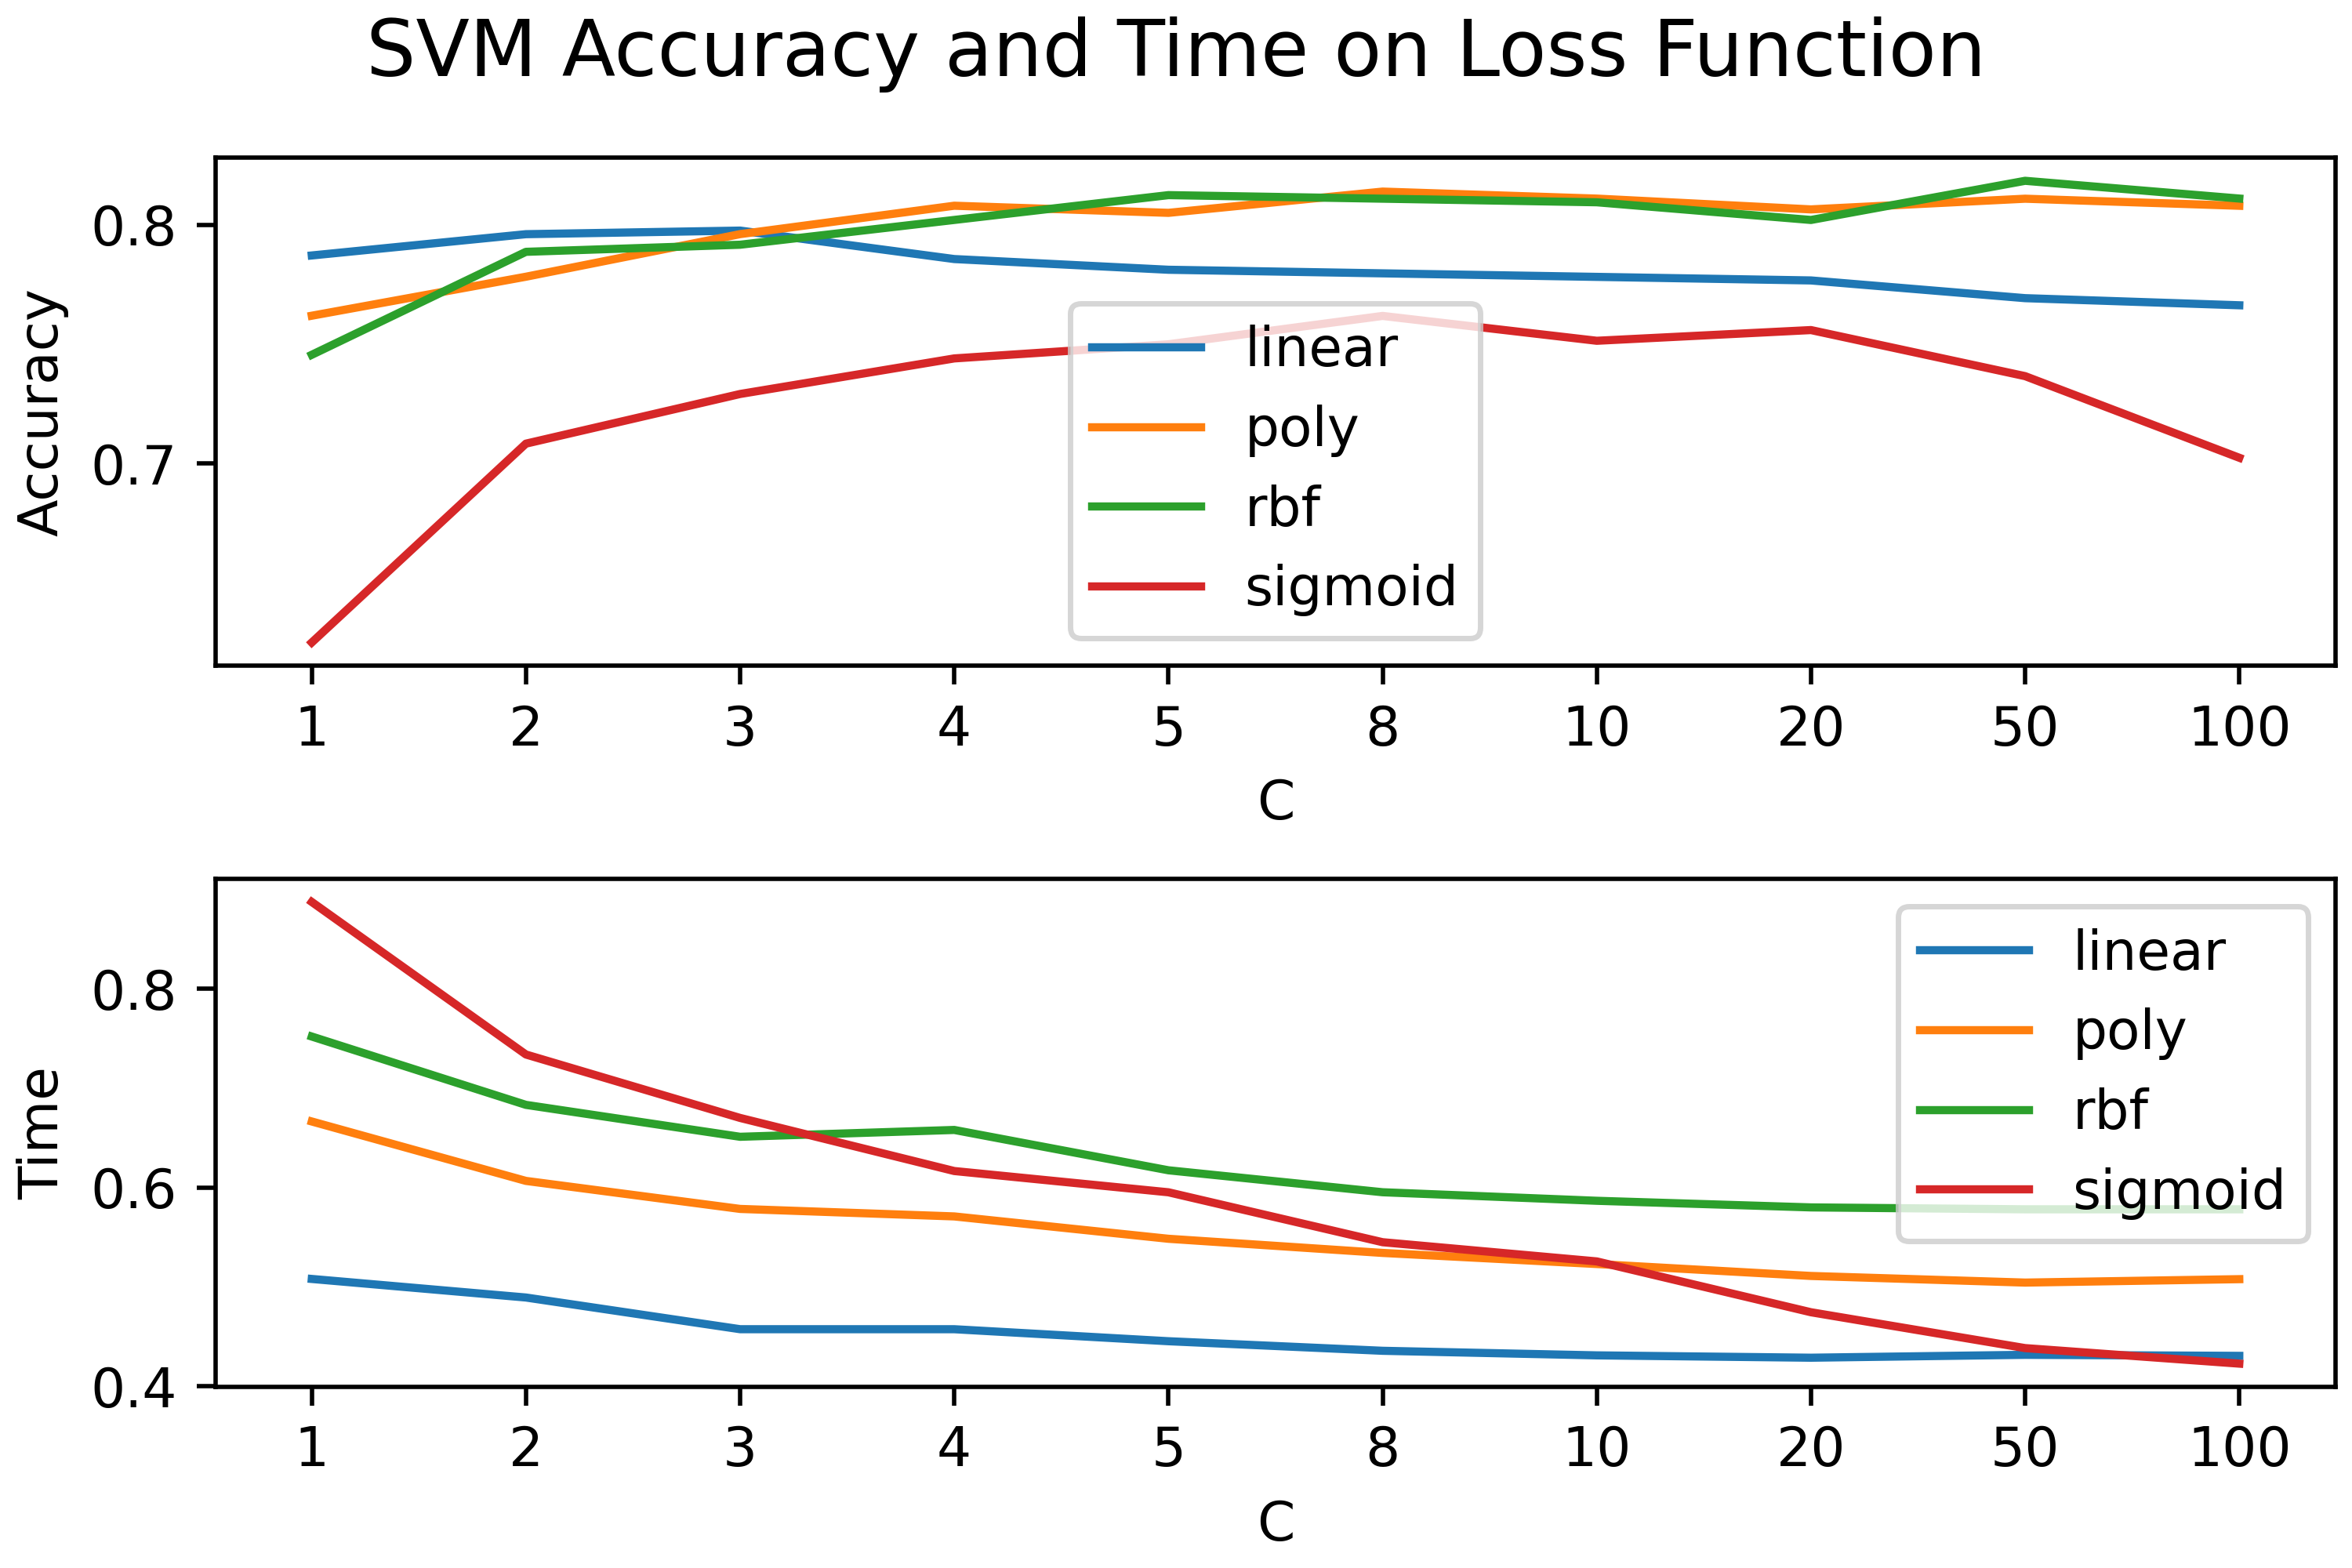
\includegraphics[width=0.65\linewidth]{images/svm_kernel.png}
                    \end{center}
                \end{minipage}
                
                % 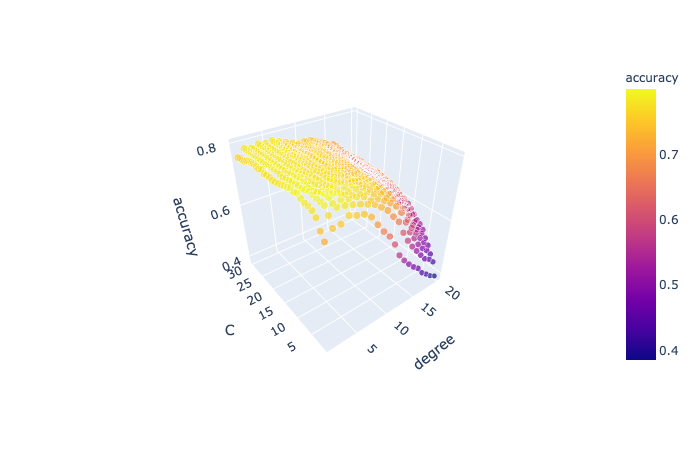
\includegraphics[width=0.75\linewidth]{images/svm_c_degree.png}
            \end{enumerate}
            Here is a summary of the hyper-parameters:
            \begin{center}
                \begin{tabular}{|c|c|}
                    \hline
                    LR&C = 5.1, penalty = $l_2$\\ \hline
                    KNN& $k = 5$\\ \hline
                    RT& Loss Function = gini, n\_estimators = 1400\\ \hline
                    SVM& Kernel = poly, degree = 2, C = 7.0\\ \hline
                \end{tabular}
            \end{center}
            \item \textbf{Prediction Results}
            \vspace{3mm}

            \begin{minipage}{0.45\textwidth}
                As shown in the Table 1, the model performing the best on the whole dataset is Random Forest classifier. When looking closely at the overall prediction results , we noticed that all models have some pattern making mistakes.
                One example is making mistakes distinguishing characters with similar hair color.
                Digging into the results with self-collected data, we found that models were easy to confuse characters with similar hair color.
                In the self-collected data set, all models made some mistakes distinguishing between \texttt{violet\_evergarden} and \texttt{saber\_arutoria\_pendoragon} since they all have blonde hair.
                About 15\% in average of \texttt{violet\_evergarden}'s images were falsely recognized as \texttt{saber\_arutoria\_pendoragon}.
                See the examples of them: Figure 13.
            \end{minipage}
            \begin{minipage}{0.3\textwidth}
                \begin{tabular}{|c|c|c|c|c|c|c|}
                    \multicolumn{7}{c}{\textbf{Non-Neural-Network Accuracies}}\\
                    \hline
                     & \multicolumn{3}{|c|}{self-collected} & \multicolumn{3}{|c|}{Whole dataset} \\ \hline
                    model & train & test & time & train & test & time \\ \hline
                    LR & 0.940 & 0.824 & $<1s$ & 0.456 & 0.335 & $38s$ \\ \hline
                    LDA  & 0.984 & 0.529 & $<1s$ & 0.422 & 0.282 & $1s$ \\ \hline
                    KNN & 0.784 & 0.739 & $<1s$ & 0.454 & 0.269 & $1m$ $56s$ \\ \hline
                    CART & 1.0 & 0.672 & $<1s$ & 0.998 & 0.218 & $9s$ \\ \hline
                    RF & 1.0 & 0.866 & $3s$ & 0.998 & 0.551 & $5m$ $8s$\\ \hline
                    NB & 0.649 & 0.462 & $<1s$ & 0.393 & 0.132 & $13s$ \\ \hline
                    SVM  & 0.946 & 0.824 & $<1s$ & 0.661 & 0.393 & $2m$ $15s$ \\ \hline
                \end{tabular}
            \end{minipage}
            
           
            \begin{figure}[h!]
                \centering
                \begin{tabular}[c]{cc}
                    \begin{subfigure}[b]{0.3\linewidth}
                        \centering
                        
\includegraphics[width=0.5\linewidth]{images/violet.png}
                        \caption{violet\_evergarden}
                    \end{subfigure} &
                    \begin{subfigure}[b]{0.3\linewidth}
                        \centering
                        
\includegraphics[width=0.5\linewidth]{images/saber2.png}
                        \caption{saber\_arutoria\_pendoragon}
                    \end{subfigure}
                \end{tabular}
                \caption{Characters with similar hair color may confuse the system}
            \end{figure}
        \end{itemize}
        \item \textbf{Non-Neural-Network Models With ResNet Last Layer Inputs}
        \begin{itemize}
            \item \textbf{Data Pre-processing and Feature Extraction}

            In this part, we directly used ResNet18, pretrained on ImageNet, as the image feature extractor. We first performed a random clip along with color normalization using the color average and standard deviation of the dataset. Then, we feed all images to the ResNet18 and use the activation values as the input. The input has a length of 1000. Before training, we also did a normalization on all vectors.
            \item \textbf{Model implementation}

            Same as the previous process, we trained a LR, LDA, KNN, CART, RF, NB, SVM classifiers.
            \item \textbf{Hyperparameter Tuning}
            
            Hyperparameters was tuned using the subset of dataset described above and the result using all of our data would also be produced after hyperparameters was tuned.
            \begin{enumerate}
                \item Logistic Regression classifier

                Similar to the previous part, we iterate over several C to see which panelty is better generally. Then we find out its cooresponding regularization strength. 

                Testing results charts: Figure 8. As shown in the charts, we select $C = 1.1, penalty = l_2$ 

                \begin{figure}[h!]
                    \begin{subfigure}[b]{0.5\linewidth}
                        \centering
                        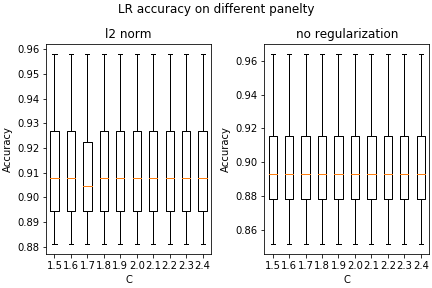
\includegraphics[width=0.8\linewidth]{images/res_tradi_LR_panelty.png}
                    \end{subfigure}
                    \begin{subfigure}[b]{0.5\linewidth}
                        \centering
                        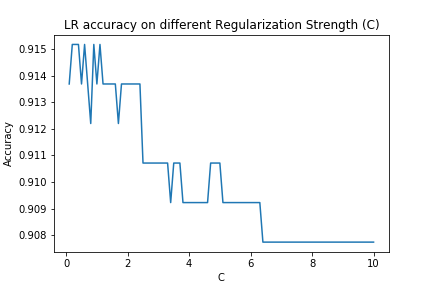
\includegraphics[width=0.8\linewidth]{images/res_tradi_LR_C.png}
                    \end{subfigure}
                    \caption{LR on ResNet Features hyperparameter tuning}
                \end{figure}
                \item K Nearest Neighbors classifier

                We tried out different values of $k$, ranging from $2$ to $30$ to find the best value of $k$.The best $k$ is 8.
                % \begin{figure}[h!]
                %     \centering
                %     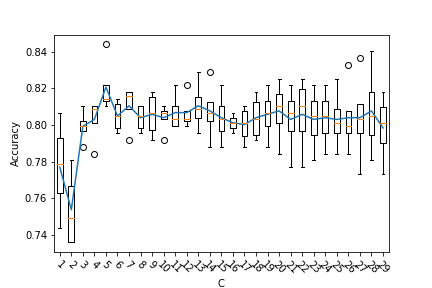
\includegraphics[width=0.5\linewidth]{images/res_tradi_KNN.png}
                %     \caption{KNN on ResNet Features hyperparameter tuning}
                % \end{figure}

                \item Random Forest classifier

                We have tried forests with different loss function, Gini impurity function and Information Entropy function, both accuracy and computing time was record. See Figure 10. As shown in the graph, we should use Gini impurity function as our loss function and the best number of estimators is $500$.

                \begin{figure}[h!]
                    \begin{subfigure}[b]{0.5\linewidth}
                        \centering
                        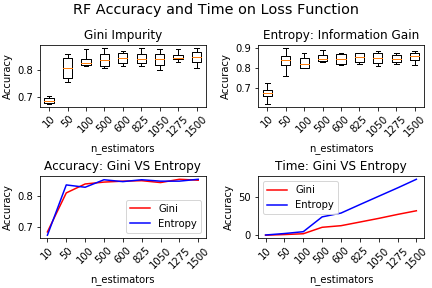
\includegraphics[width=0.7\linewidth]{images/res_tradi_RF_penalty.png}
                    \end{subfigure}
                    \begin{subfigure}[b]{0.5\linewidth}
                        \centering
                        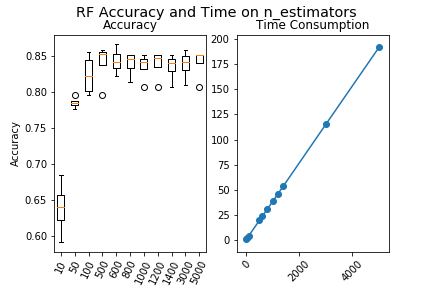
\includegraphics[width=0.7\linewidth]{images/res_tradi_RF_n_estimators.png}
                    \end{subfigure}
                    \caption{RF on ResNet Features hyperparameter tuning}
                \end{figure}

                \item Support Vector Machine classifier
                
                \vspace{3mm}

                \begin{minipage}{.4\textwidth}
                    We have tried different kernels, linear, polynomial, rbf, and sigmoid kernels to find the best kernel among them.
                    The polynomial kernel performs the best.
                    See Figure 11.
                    For polynomial kernel, we have also tried and tested different degree of polynomial kernel, ranging from $1$ to $20$, to find the best degree.
                    The regularization strength, C, was also tested with floats ranging from $1$ to $30.0$ to find the best value.
                    The best hyperparameter we have is $kernel = poly, C = 1.0$ and $degree = 4$.
                \end{minipage}
                \begin{minipage}{.4\textwidth}
                    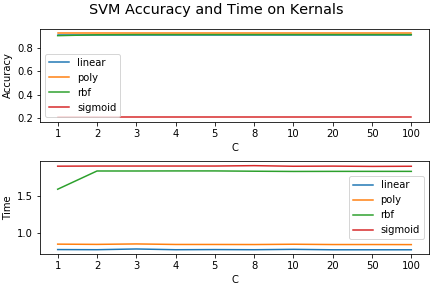
\includegraphics[width=0.8\textwidth]{images/res_tradi_SVM_penalty2.png}
                \end{minipage}
                % \begin{figure}[h!]
                %     \centering
                %     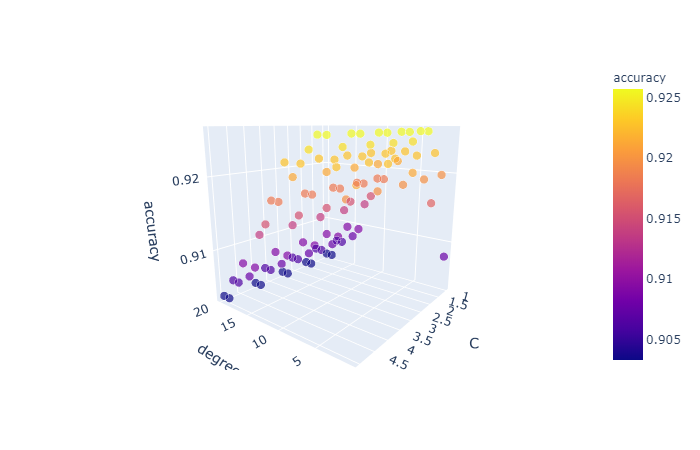
\includegraphics[width=0.75\linewidth]{images/res_tradi_SVM_c.png}
                %     \caption{SVM on ResNet Features C tuning}
                % \end{figure}

            \end{enumerate}
            Here is a summary of the hyper-parameters:
            \begin{center}
                \begin{tabular}{|c|c|}
                    \hline
                    LR&C = 1.1, penalty = $l_2$\\ \hline
                    KNN& $k = 8$\\ \hline
                    RT& Loss Function = gini, n\_estimators = 500\\ \hline
                    SVM& Kernel = poly, degree = 4, C = 1\\ \hline
                \end{tabular}
            \end{center}
            \item \textbf{Prediction Result}
            
            \vspace{3mm}
            \begin{minipage}{0.35\textwidth}
                Compared to the previous method of feature extraction, features from ResNet is performing better.
                The pattern of making mistakes between characters with, for example, similar hair color, was still persisting.
                The severity was greatly ameliorated, however.
                The result on the whole dataset is also better than the previous approach.
                All the accuracy rate on test set decreases.
                The best three model is LR, SVM and LDA
            \end{minipage}
            \begin{minipage}{0.5\textwidth}
                \begin{tabular}{|c|c|c|c|c|c|c|}
                    \multicolumn{7}{c}{\textbf{ResNet Feature Models Accuracy} }\\
                    \hline
                        & \multicolumn{3}{|c|}{self-collected} & \multicolumn{3}{|c|}{Whole dataset} \\ \hline
                    model & train & test & time & train & test & time \\ \hline
                    LR & 1 & 0.941 & 1s & 0.94 & 0.71 & 1m 10s \\ \hline
                    LDA  & 1 & 0.765 & 1s & 0.915 & 0.751 & 2s \\ \hline
                    KNN & 0.887 & 0.832 & 1s & 0.609 & 0.414 & 3m 41s \\ \hline
                    CART & 1 & 0.563 & 1s & 0.998 & 0.126 & 1m 38s \\ \hline
                    RF & 1 & 0.882 & 4s & 0.998 & 0.51 & 13m 35s\\ \hline
                    NB & 0.854 & 0.824 & 1s & 0.603 & 0.482 & 25s \\ \hline
                    SVM  & 1 & 0.908 & 1s & 0.998 & 0.679 & 3m 36s \\ \hline
                \end{tabular}
            \end{minipage}
            
            
%            \begin{figure}[h!]
%                \begin{subfigure}[b]{0.5\linewidth}
%                    \centering
%                    
\includegraphics[width=0.5\linewidth]{images/violet.png}
%                    \caption{violet\_evergarden}
%                \end{subfigure}
%                \begin{subfigure}[b]{0.5\linewidth}
%                    \centering
%                    
\includegraphics[width=0.5\linewidth]{images/saber2.png}
%                    \caption{saber\_arutoria\_pendoragon}
%                \end{subfigure}
%                \caption{Characters with similar hair color may confuse the system}
%            \end{figure}
        \end{itemize}
        \item \textbf{Neural Networks Approach (ResNet)}
        \begin{itemize}
            \item \textbf{Data Pre-processing and Feature Extraction}

            Images was loaded using \texttt{torchvision} with initial transformations of:
            \begin{itemize}
                \item randomly resizing into $224 \times 224$
                \item randomly horizontal flipping
                \item normalization using the mean and standard deviation of each RGB channel calculated from our whole dataset
            \end{itemize}

            \item \textbf{Model Implementation}

            Models were pretrained in \texttt{PyTorch}\cite{pytorch} using ImageNet so we would be starting with a good enough weight to get potential prediction improvement.
            We used cross entropy function as our loss function and stochastic gradient descent as our optimizer with initial learning rate of $0.001$, and momentum of $0.9$.
            Learning rate was also adjusted by decaying 0.1 each 7 epochs, using learning rate scheduler packaged within \texttt{PyTorch}\cite{pytorch}.
            Each model was trained for 25 epochs with training data and prediction results on both training and testing dataset were recorded after each epoch.
            \item \textbf{Prediction results}
            
            \vspace{3mm}

            \begin{minipage}{0.35\textwidth}
                We tested ResNet of 18, 34, 50, 101 layers packaged within \texttt{PyTorch}\cite{pytorch} using the subset of data mentioned above.
                The problem of distinguishing characters with similar features, e.g.\ same hair color, was persisting but was greatly ameliorated.
                Only about $12\%$ of \texttt{violet\_evergarden} was recognized as \texttt{saber\_arutoria\_pendoragon}
            \end{minipage}
            \begin{minipage}{0.45\textwidth}           
                \begin{tabular}{|c|c|c|c|c|c|c|}
                    \multicolumn{7}{c}{
                        \textbf{ResNet Accuracies}
                    }\\
                    \hline
                    & \multicolumn{3}{|c|}{self-collected} & \multicolumn{3}{|c|}{Whole dataset} \\ \hline
                    layers & train & test & time & train & test & time \\ \hline
                    18 & 0.965 & 0.969 & $1m$ $19s$ & 0.902 & 0.890 & $14m$ $48s$ \\ \hline
                    34  & 0.970 & 0.987 & $1m$ $44s$ & 0.919 & 0.900 & $24m$ $27s$ \\ \hline
                    50 & 0.964 & 0.975 & $2m$ $33s$ & 0.922 & 0.909 & $38m$ $54s$ \\ \hline
                    101 & 0.965 & 0.975 & $3m$ $59s$ & 0.936 & 0.916 & $63m$ $48s$ \\ \hline
                \end{tabular}
            \end{minipage}          
        \end{itemize}
    \end{enumerate}


    \section{Participants Contribution}
    % Please list the name of the participants. For each participant explain in details the role he/she played in the project: explain which methods was implemented by which member, which dataset was processed by which member, which experimental results were generated by which members, etc.
    \textbf{Data Collecting}: Ziqian Ge found the Nagadomi's Anime Face Character Dataset. Xin Guan did the manual data cleaning. Ziqian Ge collected the \texttt{Illyasviel\_von\_einzbern} in the self-collected dataset; Xin Guan collected the rest. \\
    \textbf{Data preprocessing}: Xin Guan did the data reforming in \texttt{data\_cleaning.py} and completed the feature extractors of Non-Neural-Network data loaders(class \texttt{feature\_extraction\_dataloader} and \texttt{resnet\_traditional\_model} in \texttt{data\_loader.py}). Ziqian Ge did the pytorch data loader and RGB information extractor (class \texttt{pytorch\_dataloader} and function \texttt{img\_stat} in \texttt{data\_loader.py}) \\
    \textbf{Model Training and Hyper parameter Tunning}: Xin Guan finished the model structures for non-neural-network models (\texttt{resnet\_traditional\_models.ipynb} and \texttt{traditional\_models.ipynb}); Ziqian Ge did the neural-network constructing and traning(\texttt{neural\_network.ipynb}). Xin Guan tuned SVM and RT's parameters along with visualization; Ziqian Ge tuned LR and KNN's parameters along with visualization. \\
    \textbf{Project Writing}: Xin Guan Completed Introduction, Technical Approach and Non-Neural-Network Models With ResNet Last Layer Inputs in Experimental Results. Ziqian Ge finished Dataset Overview, Non-Neural-Network Models with Image Features inputs and Neural-Network Model in Technical Approach along with the Participants Contribution.
    \vspace{10mm}
    % ** Please do not change the size of the fonts.

    % ** Please note that your submission must be at most 7 pages long, excluding references.

    \newpage
    \bibliographystyle{acm}
    \bibliography{ref}{}
    

    
\end{document}
